
\documentclass{article}  
\usepackage{graphicx}
\usepackage[utf8]{inputenc}
\usepackage[T1]{fontenc}
\usepackage{float}
\usepackage[italian]{babel}
\usepackage{listings}
\usepackage[usenames]{color}
\usepackage{natbib}
\usepackage{siunitx}
\usepackage[strict]{changepage}
\usepackage{physics}
\usepackage{wrapfig}
\usepackage[a4paper, top=2cm, bottom=2cm, right=2cm, left=2cm]{geometry}
\usepackage{array}
\usepackage{color}
\usepackage{colortbl}
\usepackage{amsmath}
\usepackage{amssymb}
\usepackage{multirow}
\usepackage{enumitem}
\usepackage{hyperref}
\usepackage{times}
\usepackage{booktabs}
\usepackage{subfig}
\usepackage{multirow}



\title{Effetto Zeeman}
\author{Docente: dott. Garfagnini, dott. Lunardon \\
	Gruppo 14}
\date{Anno accademico 2019/20}

\begin{document}
	
	
	
	\maketitle
	
	\begin{itemize}
		\item[$\circ$] Aidin Attar - 1170698 - aidin.attar@studenti.unipd.it
		\item[$\circ$] Ema Baci - 1171107 – ema.baci@studenti.unipd.it
		\item[$\circ$] Alessandro Bianchetti – 1162147 – alessandro.bianchetti@studenti.unipd.it
	\end{itemize}
	
	\vspace{3 cm}
	\begin{large}\textsc{\textbf{Scopo dell'esperienza}: studio dell'effetto Zeeman per  l'atomo di Neon, stima del fattore di Landè} 
	\end{large}
	\vspace{8.5cm}
	
	\begin{figure}[H]
		\centering
	
\includegraphics[scale = 0.5 , angle=0]{unipd_logo.png}
	\end{figure}
	
	%\newpage \tableofcontents \newpage
	
	\twocolumn
	
	\subsection*{Descrizione dell'apparato} 
	
	L'apparato sperimentale si compone di una lampada al Neon, capace di emettere
	radiazione elettromagnetica associata principalmente a transizioni tra 3p e 2p.
	In particolare siamo interessati alla transizione da $\lambda = $585.3 nm.
	Tale lampada è inserita all'interno di una cavità magnetica, per cui ci si 
	aspetta la comparsa di tre righe di emissione: tuttavia, considerando la 
	polarizzazione delle righe, possiamo “sopprimere” la transizione centrale
	orientando il campo magnetico in modo longitudinale alla linea di 
	osservazione, in modo tale da vedere solo le due righe marginali. 
	
	Il raggio di luce emessa attraversa una lente condensante, necessaria 
	per concentrare quanto più possibile il fascio, che passa quindi per una 
	fenditura e successivamente attraverso un prisma, necessario per ruotare di 
	$90 ^{\circ}$ la luce e dividerla nelle sue componenti principali. 
	
	A questo punto i raggi incidono sulla lamina di Lummer-Gehrcke, dispositivo
	interferenziale ad alta risoluzione, in modo quasi
	radente (faremo in seguito una stima dell'angolo di incidenza) e il fascio 
	emergente viene infine focalizzato sul dispositivo ottico di lettura (un CCD
	monodimensionale) attraverso la lente di camera.
	
	%La presa dati di questa esperienza è stata svolta interamente da remoto; in 
	%particolare la connessione al PC del laboratorio avviene tramite 
	%l'esportazione dello schermo via VNC Viewer.
	
	L'acquisizione dei dati è avvenuta tramite l'interfaccia di controllo dell'apparato, che permette di controllare le diverse componenti appena citate.
	
	Per l'analisi dati sono stati utilizzati programmi scritti in c++, root ed Excel.
	
	\subsection*{Compendio di teoria}
	
	L'esperienza è incentrata sull'identificare e misurare lo splitting 
	Zeeman dei livelli di energia e confrontarli con le previsioni teoriche. L'effetto Zeeman è il fenomeno che si verifica nel momento in cui gli
	atomi di una certa sostanza vengono sottoposti a un campo magnetico 
	esterno, che suddivide i livelli energetici permessi per gli elettroni.
	In tal modo confrontando lo spettro della prima riga di transizione 
	($\lambda = $585.3 nm, associata ai termini spettroscopici
	$^1S^0 \rightarrow {}^1P^1$ ) a campo magnetico spento e a campo 
	acceso vedremo 
	il biforcarsi delle campane in due ulteriori picchi. Misurando la
	distanza che separa i due picchi causati dalla presenza del campo,
	otterremo il doppio dello splitting $\Delta\lambda_{Zee} $.
	
	In particolare, si sceglie la transizione indicata sopra perché connette
	stati con spin nullo, per cui ci assicura l'effetto
	Zeeman cosiddetto \textit{normale}, cioè quello previsto anche dalla 
	teoria classica, dove il fattore giromagnetico presente nella formula 
	generale (effetto Zeeman \textit{anomalo}) sarà dunque semplicemente
	$g_l = 1$. Pertanto
	
	\begin{equation}
		\Delta E_{Zee} = g_l m \mu_B B = \pm \mu_B B
	\end{equation}
	
	
	dato che nel nostro caso le due proiezioni del momento angolare totale
	dello stato di arrivo possibili sono $m = \pm 1$ (0 è escluso grazie all'
	orientazione del campo magnetico, come accennato sopra).
	
	Inoltre
	
	\begin{equation}
		\Delta\lambda_{Zee} = \frac{\lambda^2}{hc}\Delta E_{Zee}
	\end{equation}
	
	rappresenta la formula con cui confronteremo il dato sperimentale
	ricavato.
	
	Inoltre da opportuni fit dei picchi ricaveremo una stima della larghezza
	delle campane, da cui si ottiene il potere risolvente come rapporto
	
	\begin{equation}
		R = \frac{\lambda}{\Delta\lambda}    
	\end{equation}
	
	che sarà ben coperto dalla risoluzione dell'apparato, cioè dalla
	risoluzione offerta dalla lamina di Lummer-Gehrcke, che segue l'ordine
	del rapporto L/$\lambda$, dove L è la lunghezza della lamina.
	Un altro parametro importante della lamina è il \textit{range di 
		lunghezza d'onda utile} $\Delta\lambda_{r.u.}$, che rappresenta la
	massima differenza tra due lunghezze d'onda tale che i due massimi 
	consecutivi restino distinguibili. In particolare
	
	\begin{equation}
		\label{eqn:dlru}
		\Delta\lambda_{r.u.} = \frac{\lambda^2}{2d}\frac{\sqrt{n^2-\sin(i)^2}}{n^2-\sin(i)^2-n\lambda\frac{dn}{d\lambda}}
	\end{equation}
	
	dove la derivata $dn/d\lambda$ è stata ottenuta fittando alcuni punti 
	n($\lambda$) rappresentativi dell'andamento dell'indice di rifrazione
	della lamina in funzione della lunghezza d'onda. Nello specifico si è
	scelto il modello della legge di Cauchy fermandosi al primo ordine:

	\begin{equation}
		n(\lambda) = A + \frac{B}{\lambda^2}    
	\end{equation}


	ottenendo il seguente andamento:
	
\begin{center}
	\begin{figure}[ht]
		\centering
		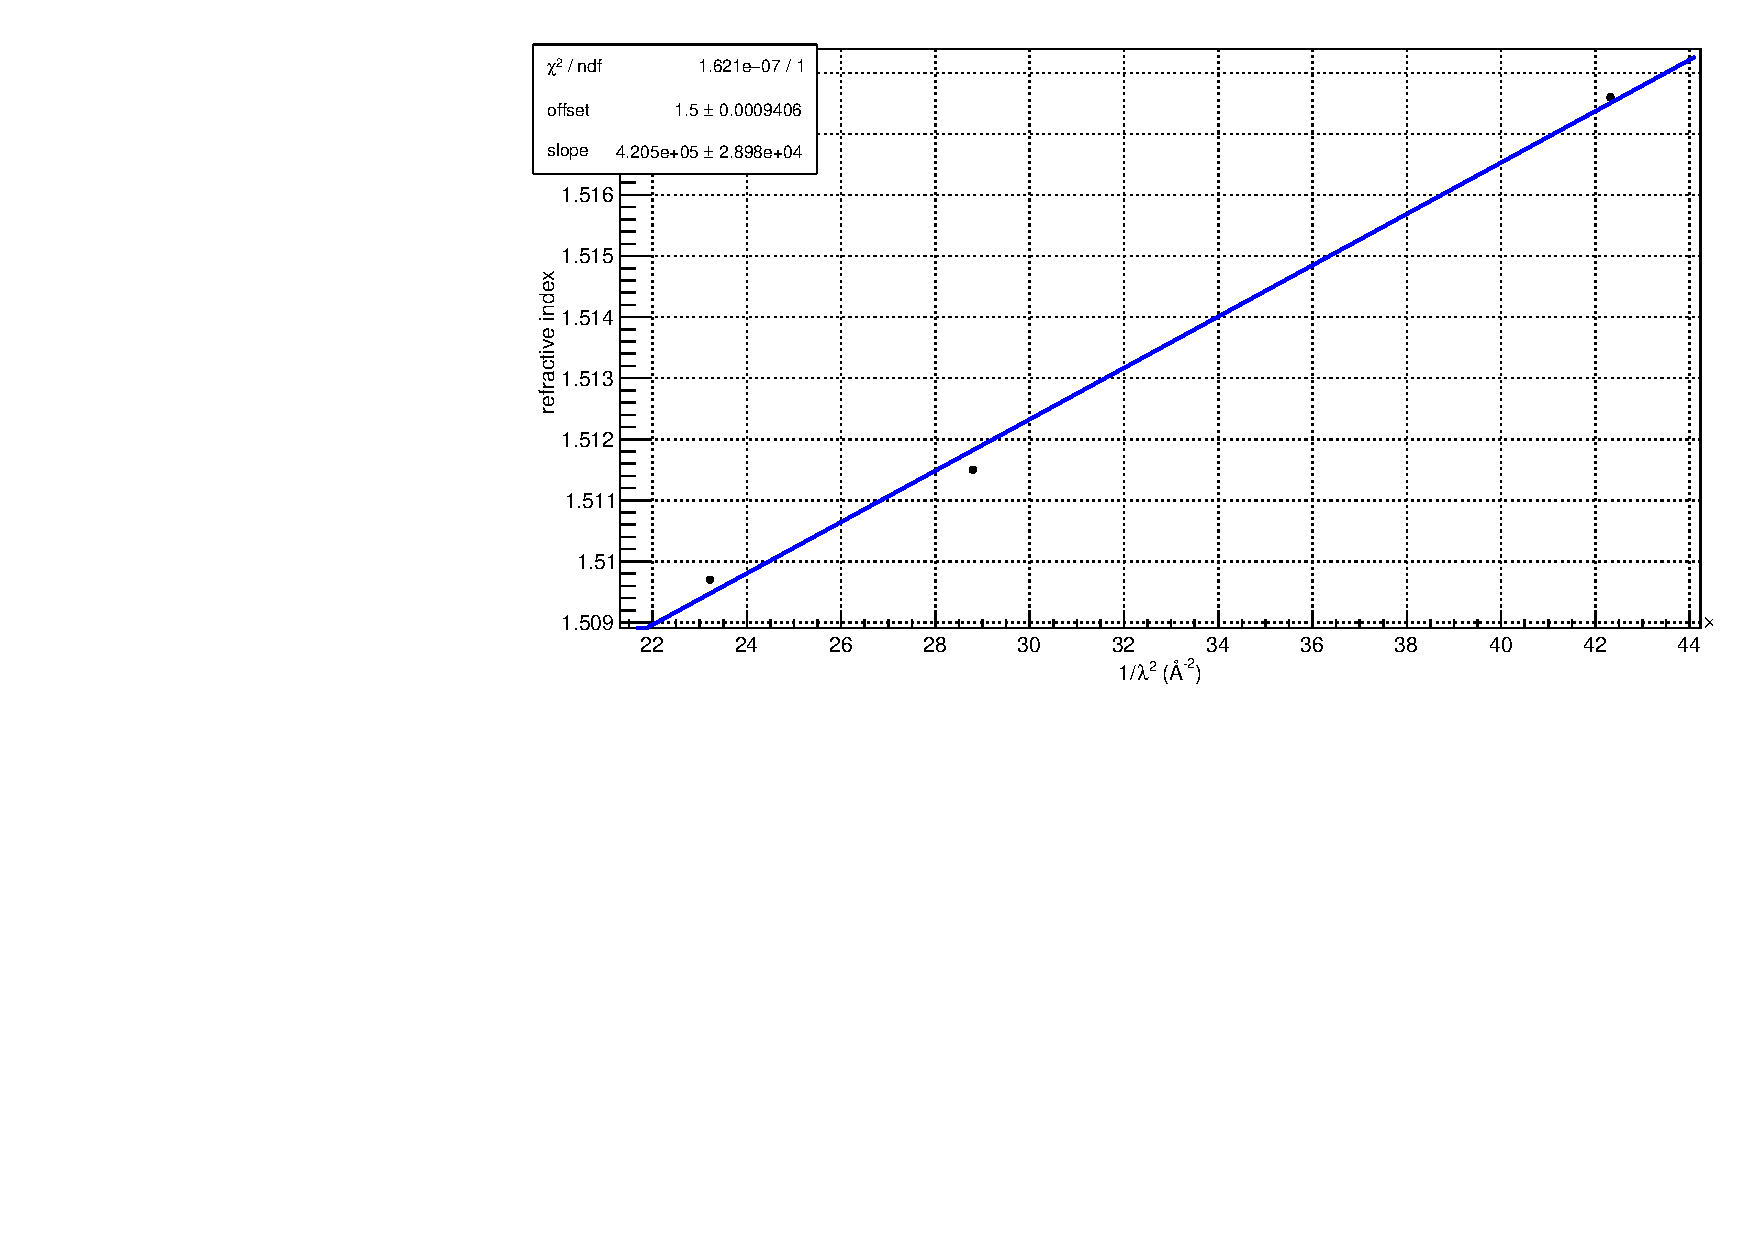
\includegraphics[scale=0.38, angle=0]{nFit.pdf}
        \setlength{\belowcaptionskip}{-20pt}
		\caption{ indice di rifrazione}
		\label{fig:nFit}
	\end{figure}
\end{center}

si riporta inoltre anche il grafico dei residui:
\begin{center}
	\begin{figure}[ht]
		\centering
		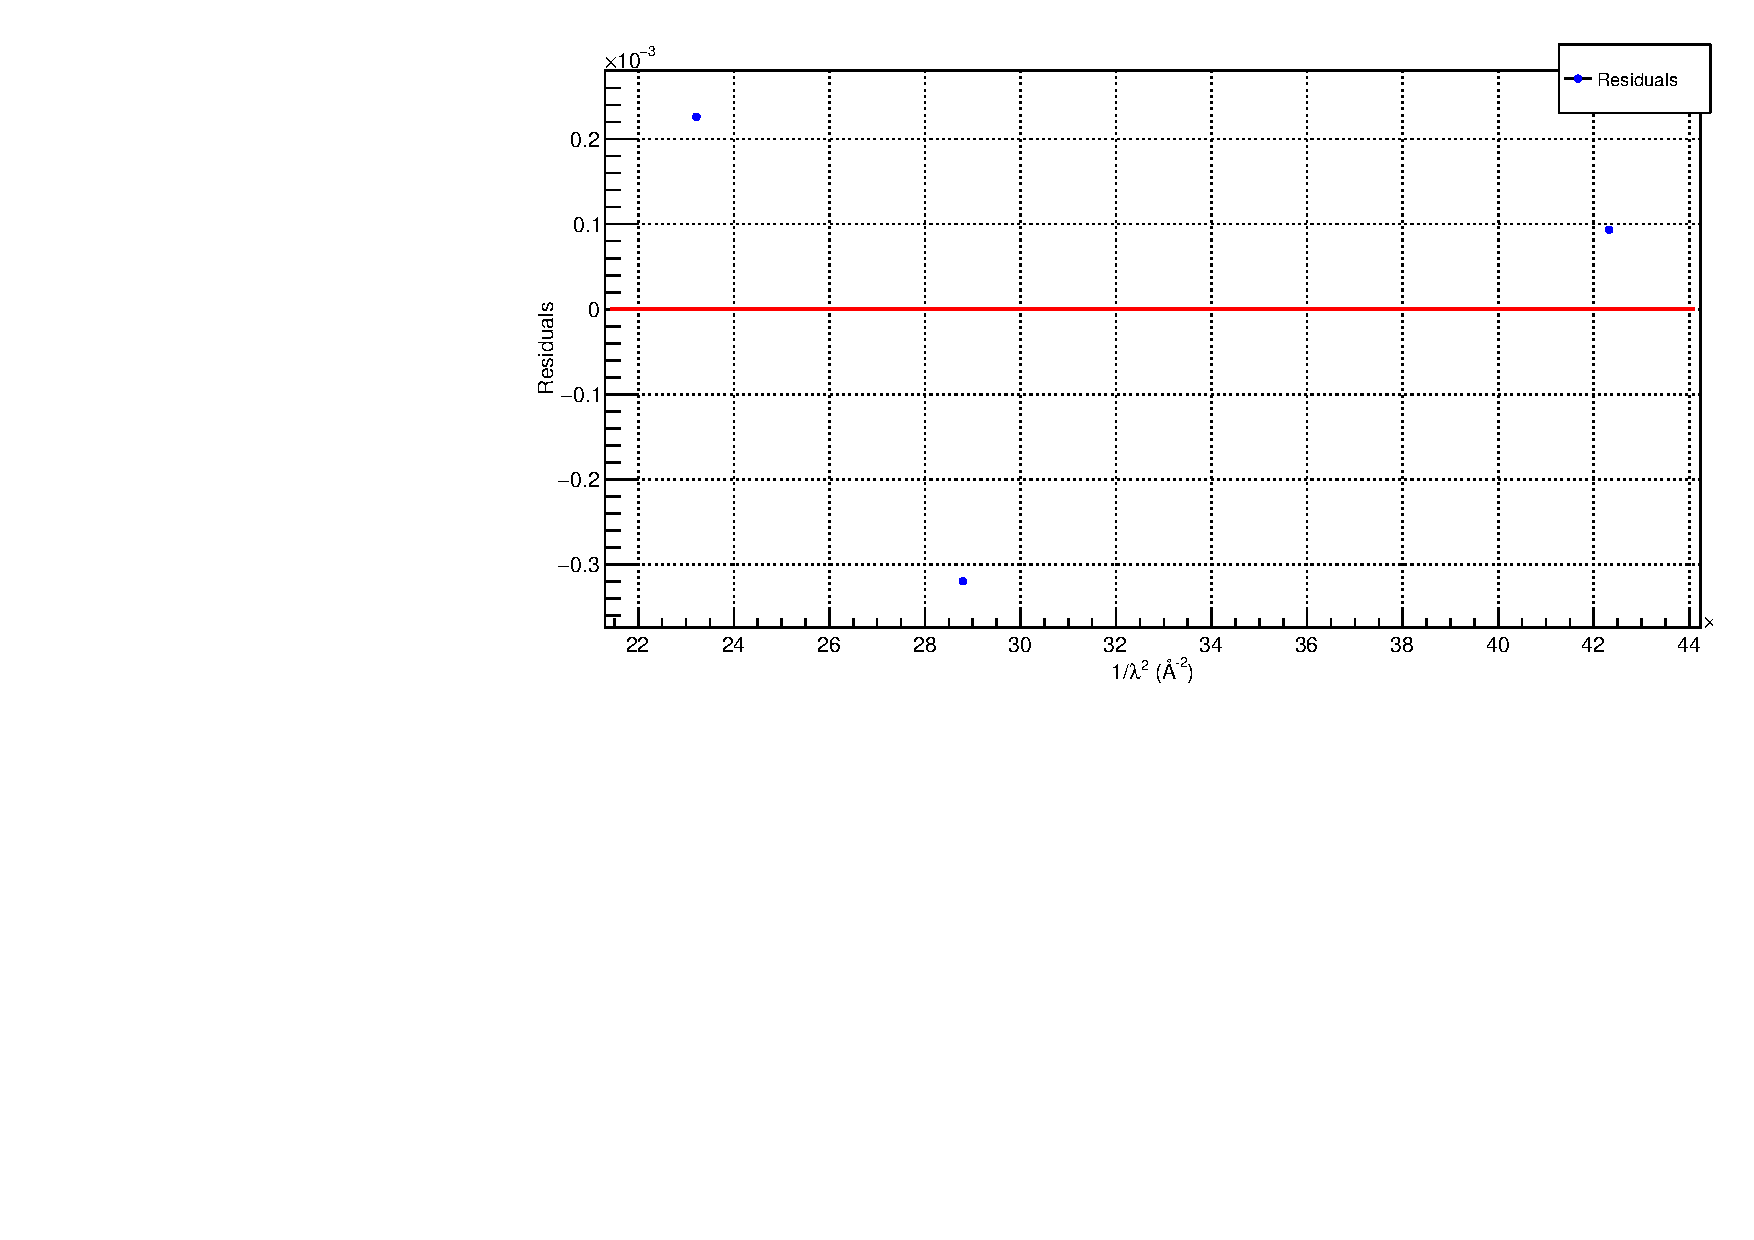
\includegraphics[scale=0.38, angle=0]{nFitRes.pdf}
        \setlength{\belowcaptionskip}{-20pt}
		\caption{ Andamento dei residui}
		\label{fig:nFitRes}
	\end{figure}
\end{center}

	I parametri del fit sono :
	$$ A= 1.4997 \pm 0.0009 \quad B= (42 \pm 3 )\cdot 10^4 \text{m}^2$$
	Per $\lambda= 585.3$ nm si ottiene quindi :
	$$n(\lambda)= 1.512 \pm 0.001  $$
	$$  \frac{dn}{d\lambda} = (-4.19 \pm 0.03 )\cdot 10^{-5} \text{m}^{-1}$$

	\section*{Aquisizione dati}
	
	\paragraph{Calibrazione}
	Prima di procedere con la presa dati si è eseguita una calibrazione 
	dell'apparato; in particolare occorre regolare la posizione 
	della sorgente rispetto all'apertura della fenditura.
	Il primo passaggio è stato quindi impostare l'apertura della fenditura 
	a $24 \mu$m ed acquisire un primo spettro a lamina disinserita, con il 
	CCD orizzontale. Zoomando sui primi 3/4 picchi dello spettro, saremo
	in grado di individuare il nostro picco di interesse.
	Successivamente si è regolata ulteriormente la posizione della sorgente 
	cercando quella che massimizzasse l'intensità e la forma del picco di 
	interesse.
	Si è quindi fissata la posizione del CCD a 0.93 mm e impostata l'apertura 
	della fenditura a $18 \mu$m.
	Infine si sono regolate le posizioni della lente focale e della lente 
	condensante, scegliendo come posizioni ottimali rispettivamente 15.36 mm 
	e 14.62 mm.


	\subsection*{Campo magnetico spento}

	Dopo la calibrazione si è proseguito con l'acquisizione del primo 
	spettro a campo magnetico spento: dopo aver selezionato il picco di 
	interesse si è inserito la lamina di Lummer-Gerhcker, e selezionato 
	con i cursori il range dello scanning, si è ruotato il CCD
	in posizione verticale.
	Infine si è impostato un tempo di integrazione di 600 ms e si è avviato
	lo scanning, dopo aver salvato il file nell'opportuna cartella.


	\paragraph{Analisi dello spettro}
	Per procedere con l'analisi dello spettro, si è caricata ed eseguita su root la macro ReadZeemanImage.C. 
	Si è ottenuto quindi un istogramma bidimensionale, al quale si è sottratto il segnale di fondo riferendosi alla sua proiezione 
	sull’asse x.
	Dopo aver sottratto il fondo, migliorando la nitidezza dell'immagine, si sono registrati i limiti della zona del segnale. 
	In questo modo si è quindi ottenuta anche la proiezione di tale regione sull’asse y, in cui si osservano una serie di picchi, 
	di cui si può migliorare la pulizia dell'immagine mediante un rebin.

	\begin{center}
		\begin{figure}[H]
			\centering
			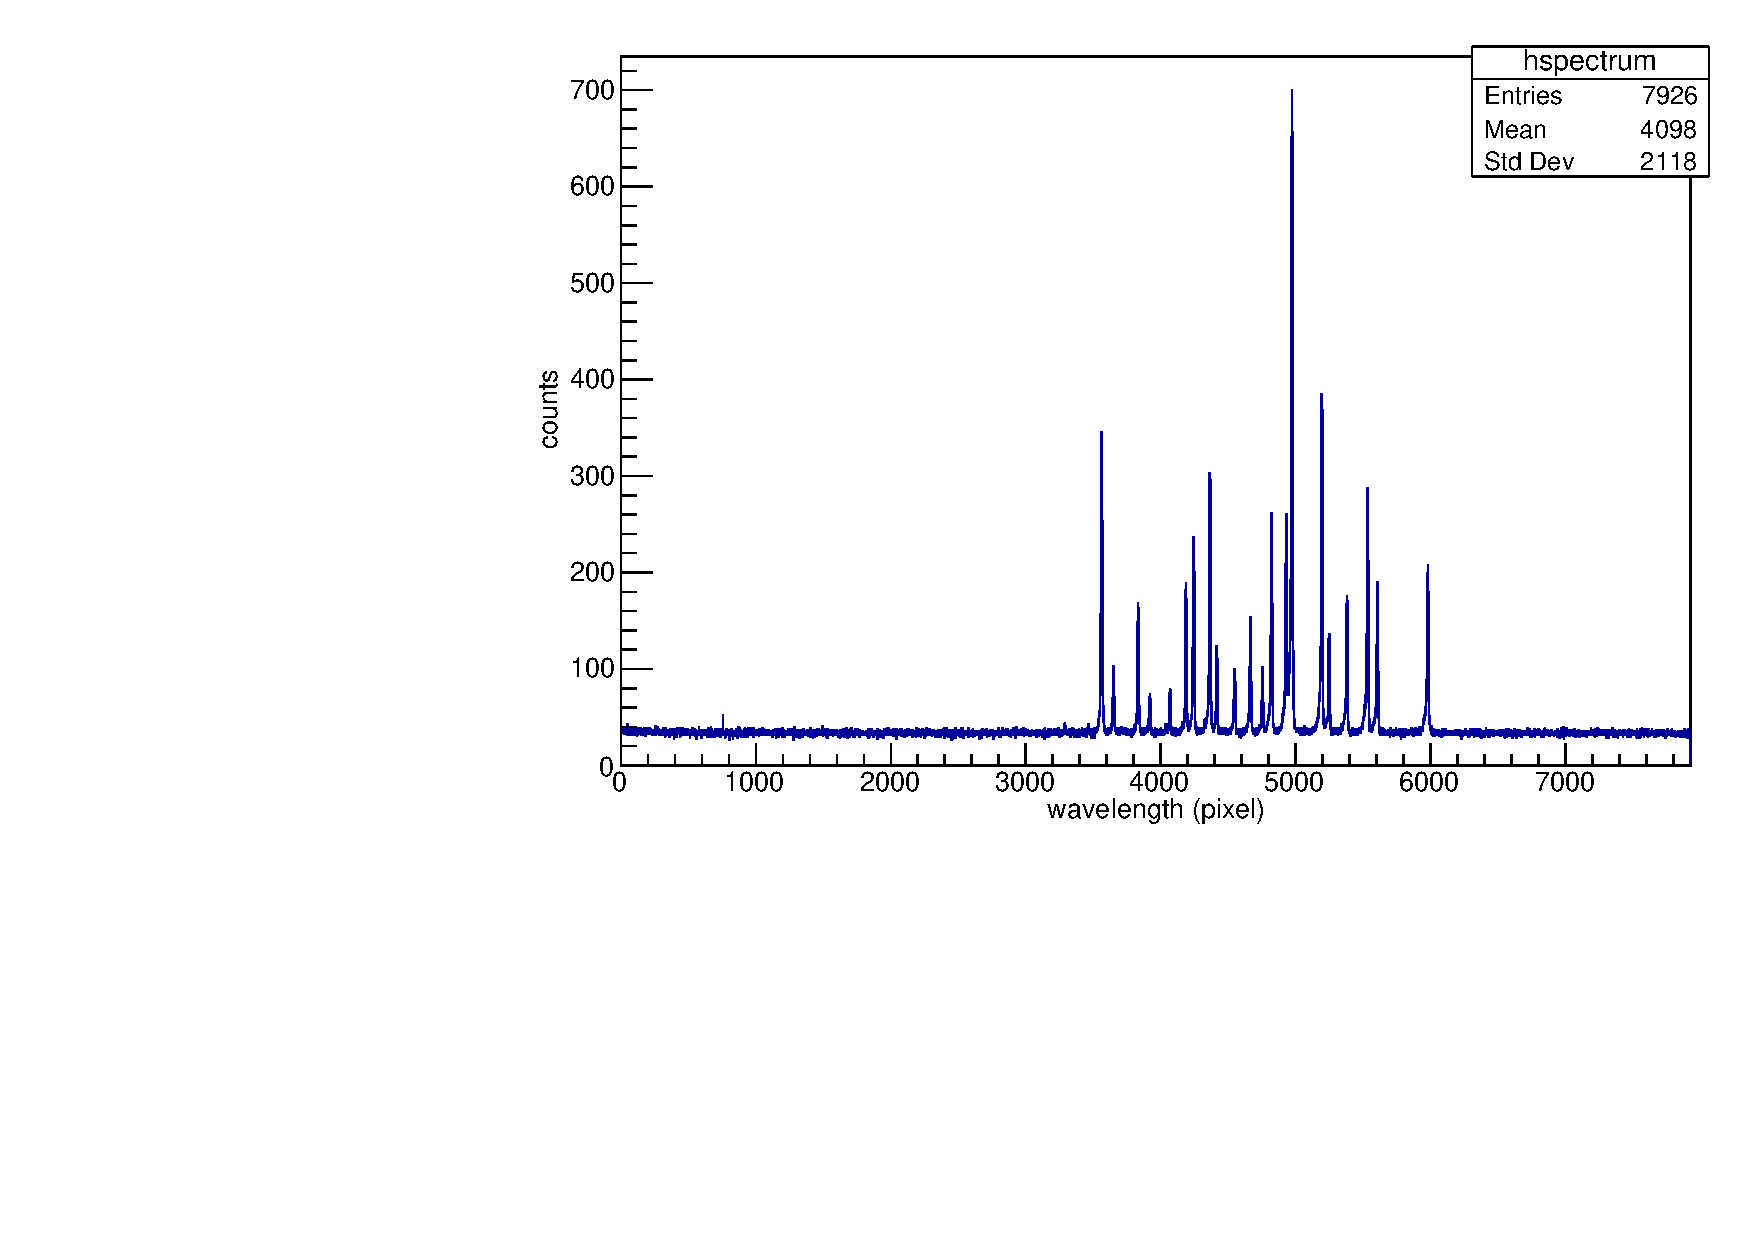
\includegraphics[scale=0.38, angle=0]{spectrum.pdf}
			\setlength{\belowcaptionskip}{-20pt}
			\caption{Spettro completo}
			\label{fig:spectrum}
		\end{figure}
	\end{center}

	\begin{center}
		\begin{figure}[H]
			\centering
			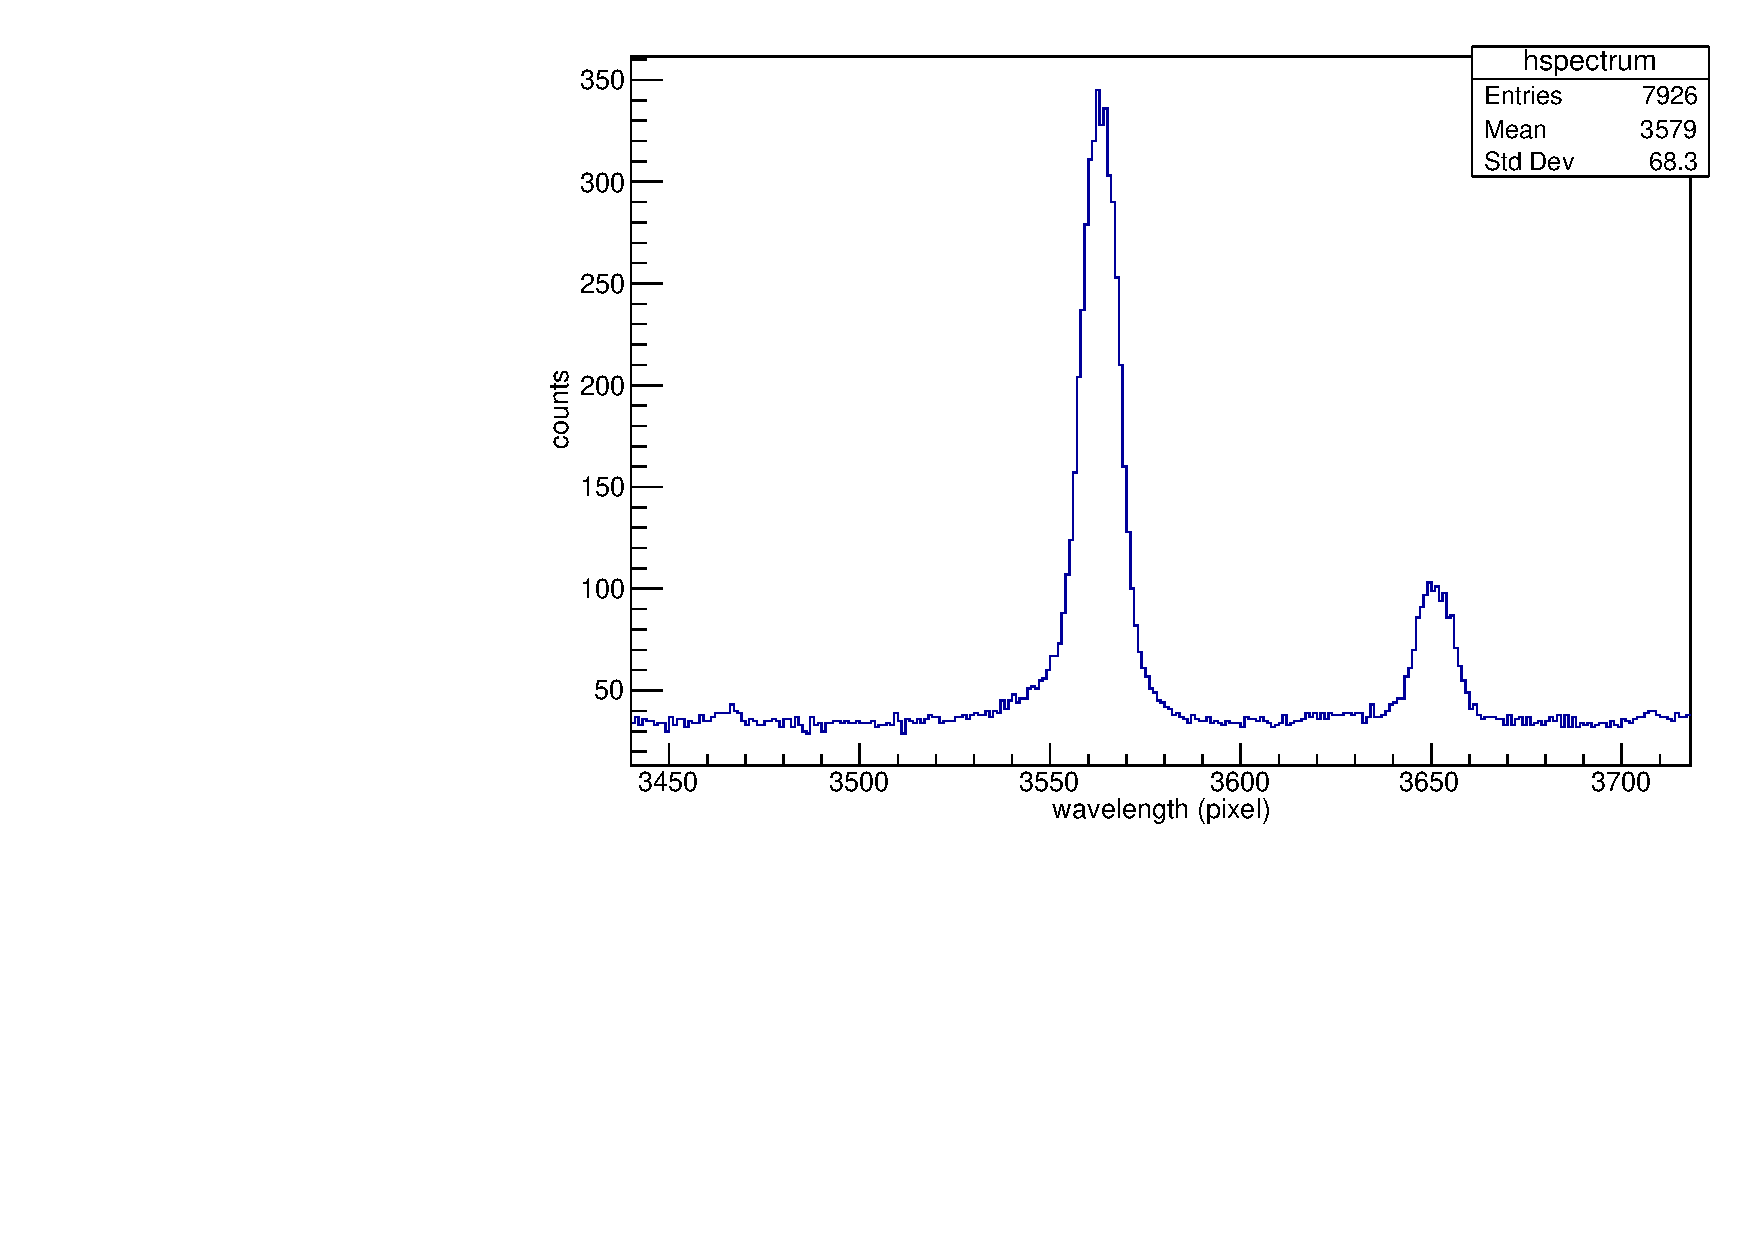
\includegraphics[scale=0.38, angle=0]{zoomspectrum.pdf}
			\setlength{\belowcaptionskip}{-20pt}
			\caption{Zoom sulle righe in esame}
			\label{fig:spectrumzoom}
		\end{figure}
	\end{center}



	\paragraph{Analisi dei picchi}


	Per fornire un'analisi estesa dello spettro si è scelto di suddividerlo  in 6 terne di picchi consecutivi, e per ciascuna terna
	l'obiettivo è studiare le spaziature tra i picchi e caratterizzarne in
	qualche modo la larghezza. 
	In particolare si è scelto di eseguire un fit gaussiano sui picchi
	per poter individuare con precisione l'ordinata di massimo e per
	poter dare una stima della larghezza del picco come FWHM.
	
	Riportiamo come esempio il seguente grafico in cui si è scelto di fittare solo uno dei  tre picchi per semplicità:
	
	\begin{center}
		\begin{figure}[H]
			\centering
			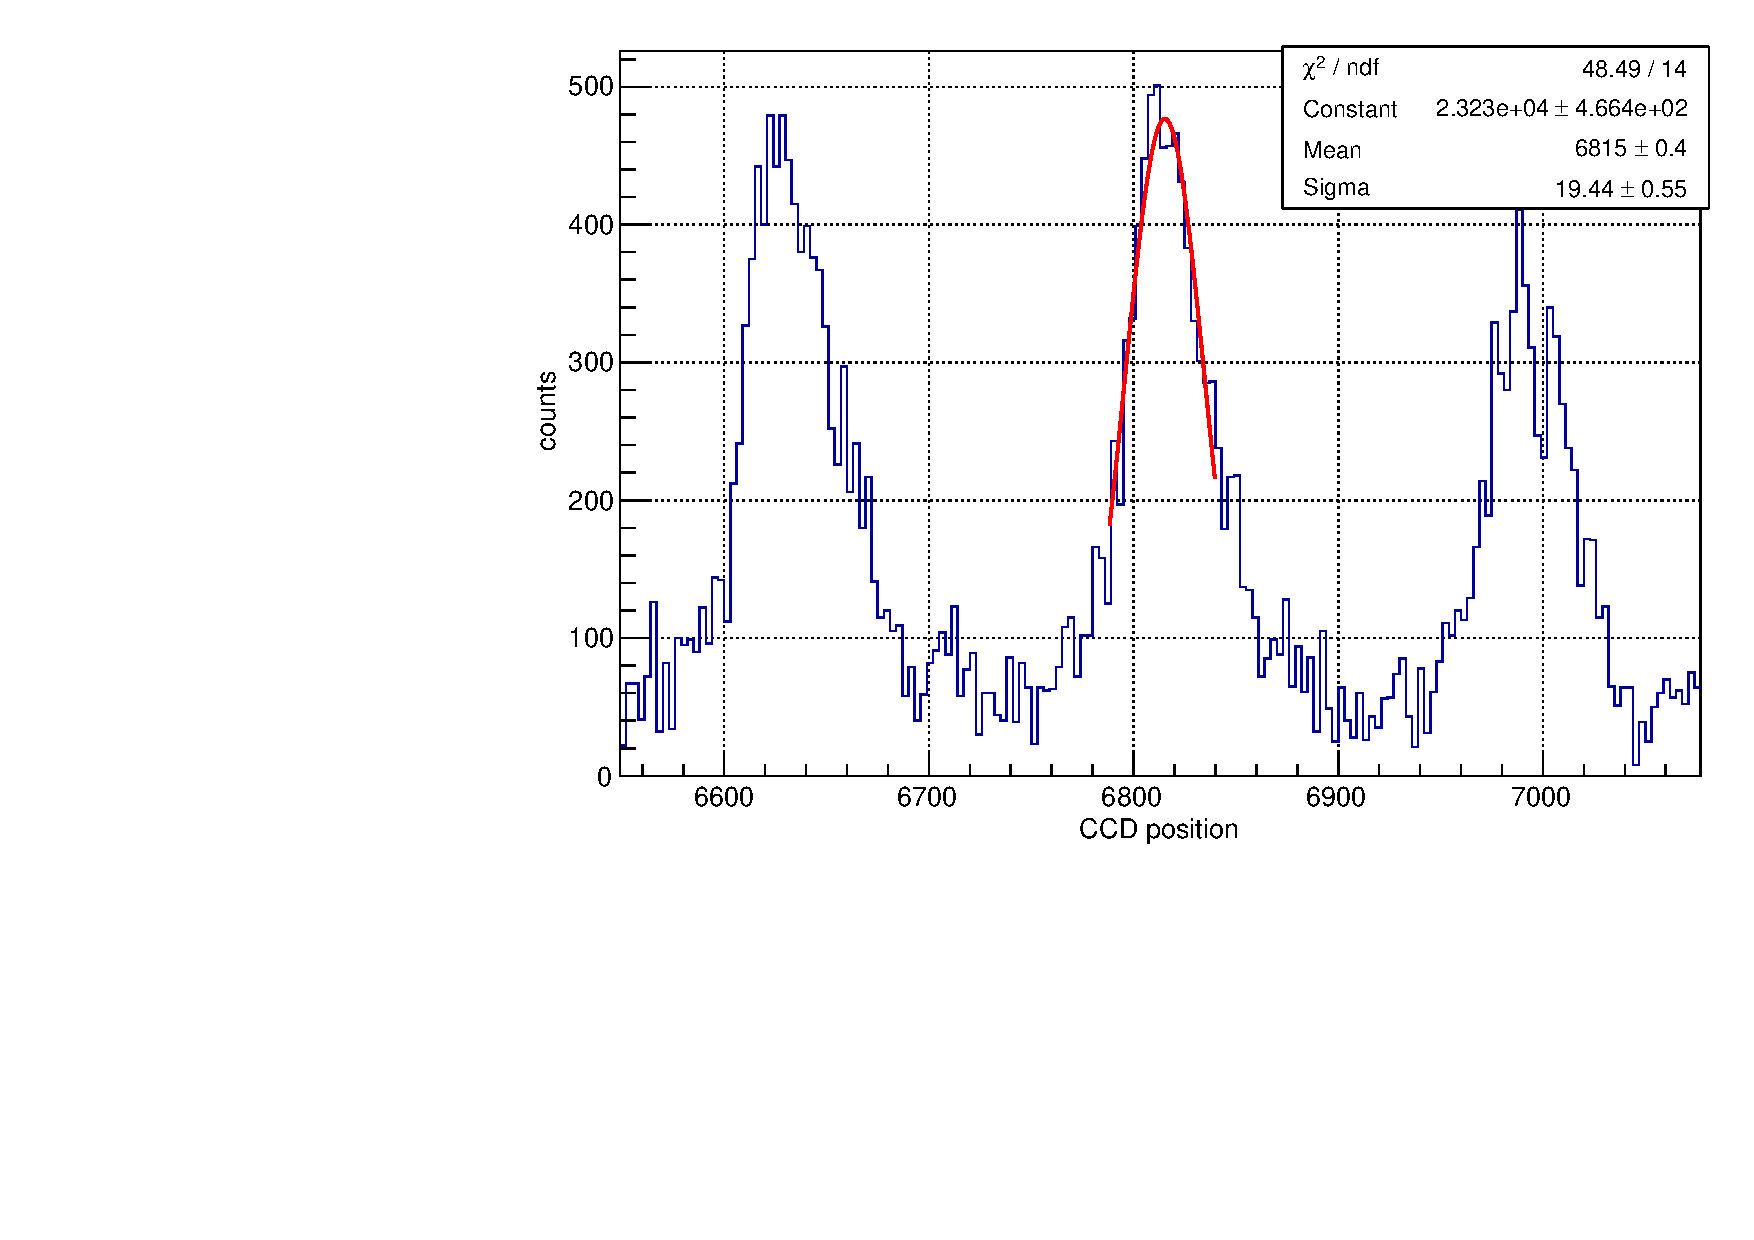
\includegraphics[scale=0.38, angle=0]{campospento/singolo.pdf}
			\setlength{\belowcaptionskip}{-20pt}
			\caption{ Esempio di fit gaussiano nel caso senza campo magnetico}
			\label{fig:singoloBoff}
		\end{figure}
	\end{center}
	
	Si noti il valore del $\chi^{(2)}$ incompatibile con il valore di aspettazione, 
	con compatibilità $\lambda \approx 6.5$. Si è notato che il valore del $\chi^{(2)}$
	risulta molto influenzato dalla scelta del range di interpolazione. Alla luce di questa
	dipendenza, si è cercato di trovare il giusto equilibrio tra una sufficiente
	larghezza di range e un buon valore di $\chi^{(2)}$, per evitare di fare fit troppo
	stretti che avrebbero sì migliorato il valore dell'estimatore ma al contempo avrebbero 
	perso informazioni sulla stima della larghezza.
	Infatti i valori dell'estimatore ottenuti dai vari picchi suggeriscono compatibilità 
	in alcuni casi e non in altri.


	Per prima cosa, studiamo l'andamento delle spaziature tra i picchi. 
	Per ciascuna terna, si sono calcolate le due distanze tra i valori medi
	delle tre gaussiane, considerandone poi la media aritmetica $\Delta x_{ru}$,
	disponendo così di un valore univoco per ciascuna terna.
	In particolare ci si aspetta per queste distanze un andamento quadratico 
	in funzione della posizione del CCD. Si è effettuata dunque un'interpolazione
	parabolica, con il fine di stimarne poi l'ordinata di vertice che 
	costituirebbe la distanza minima efficace da usare per la stima
	corretta dell'angolo di incidenza i. Tale stima corretta di i
	permette di calcolare $\Delta\lambda_{ru}$ evitando l'approssimnazione $i \approx \pi$/2. 
	Maggiori dettagli sono riportati alla fine di questa sezione.
	Avendo a disposizione il valore medio della spaziatura tra i picchi per ciascuna
	terna, si è calcolato il fattore di calibrazione valido per quella regione
	di spettro, secondo il rapporto

	\begin{equation}
		F = \frac{\Delta\lambda_{ru}}{\Delta x_{ru}}.
	\end{equation}

	Il fattore di calibrazione F rappresenta il fattore di conversione da pixel, 
	ossia l'unità di misura caratteristica del CCD, in metri.

	%CONTINUO QUI NESSUNO SI PERMETTA



	\paragraph{Stima dell'angolo di incidenza sulla lamina di Lummer-Gehrcker}
	Si è accennato in precedenza che i raggi di luce incidono quasi radenti
	alla lamina. In particolare è possibile effettuare una stima precisa dell'angolo
	di incidenza. Occorre innanzitutto calcolare l'apertura angolare
	$\Delta i$, pari al rapporto $\Delta x_{ru}$/f, dove f = 0.25 m è la distanza
	focale della lente e il valore di $\Delta x_{ru}$ è ottenuto dall'ordinata 
	di vertice del fit parabolico, cioè $y_{min} = a - b^2 / 4c$ nella 
	parabola $y = a +bx + cx^2$.


	\begin{center}
		\begin{figure}[H]
			\centering
			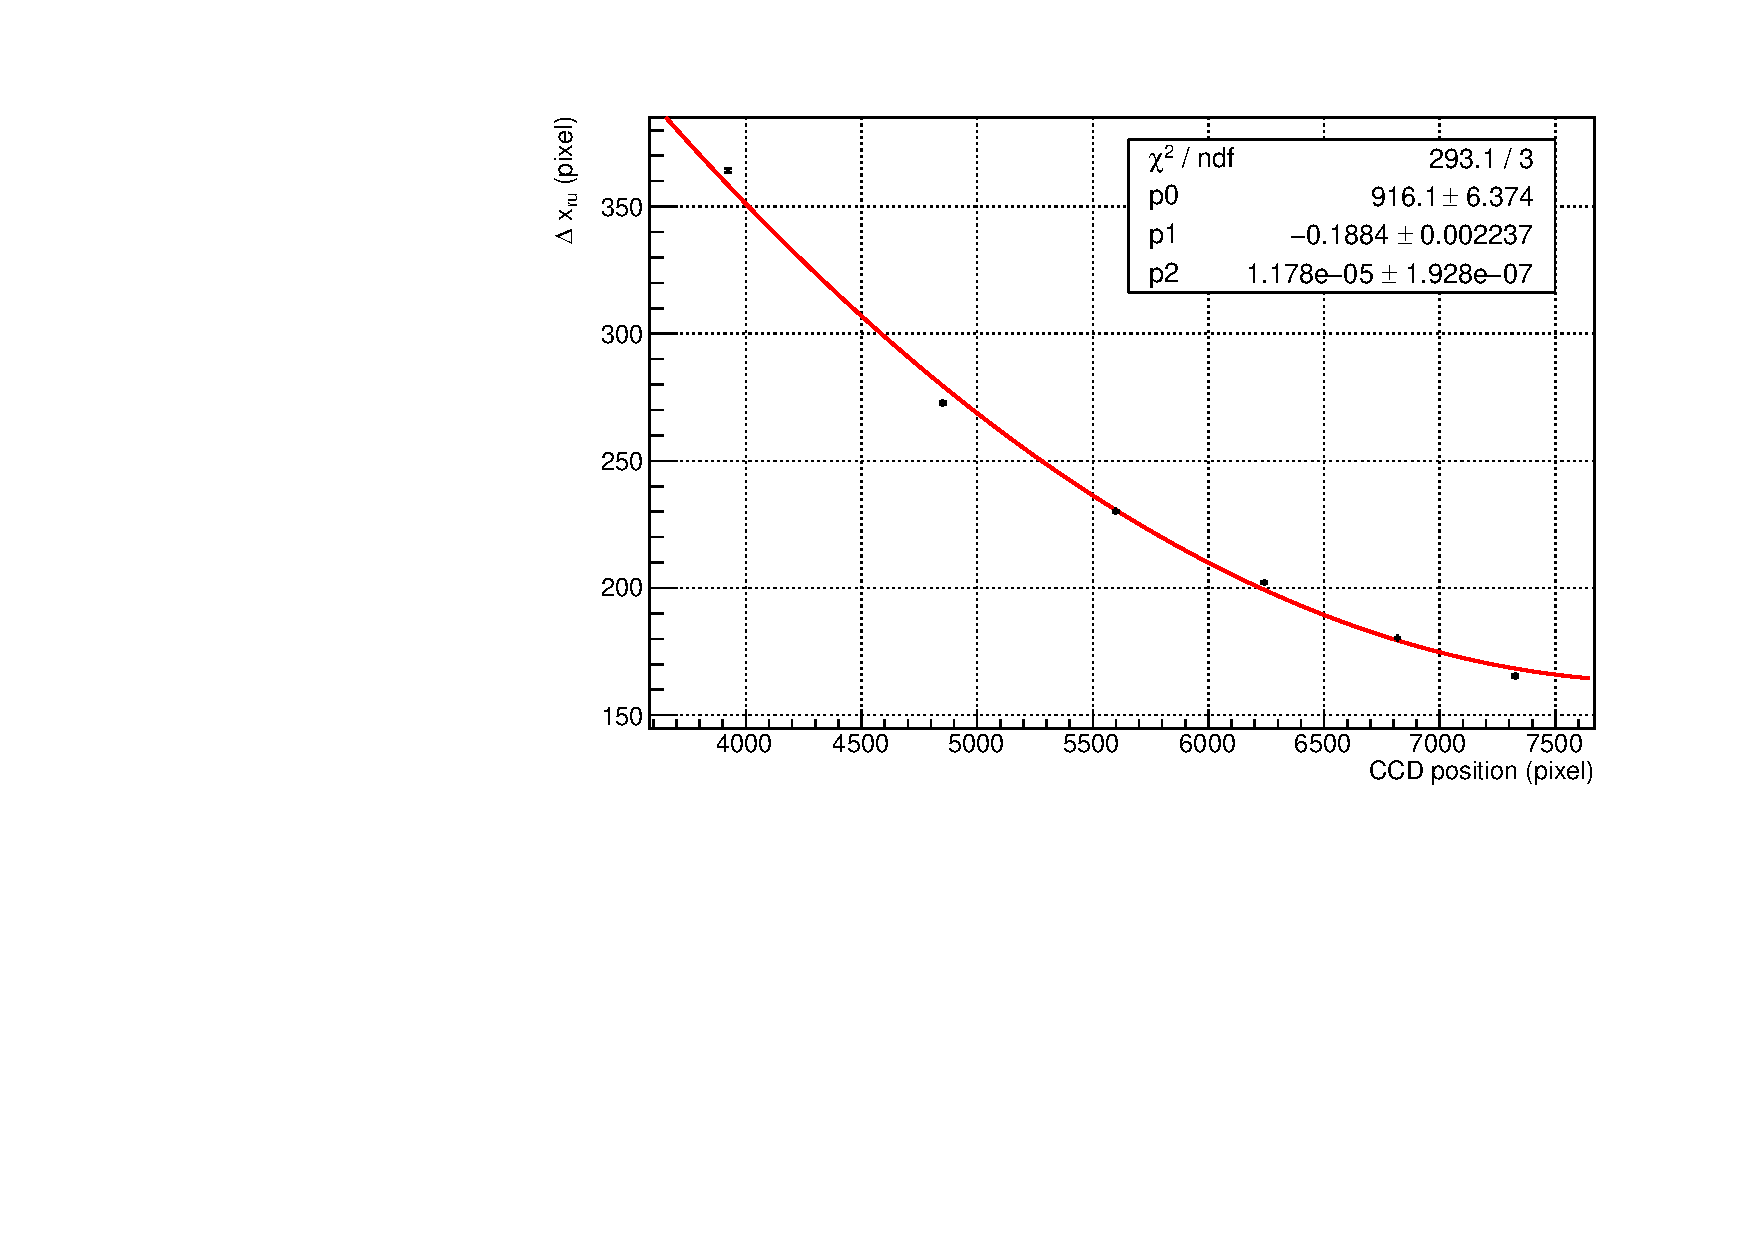
\includegraphics[scale=0.38, angle=0]{campospento/deltaxruBoff.pdf}
			\setlength{\belowcaptionskip}{-20pt}
			\caption{Andamento delle spaziature tra i picchi rispetto alla posizione del CCD}
			\label{fig:deltaxruBoff}
		\end{figure}
	\end{center}

	\begin{center}
		\begin{figure}[H]
			\centering
			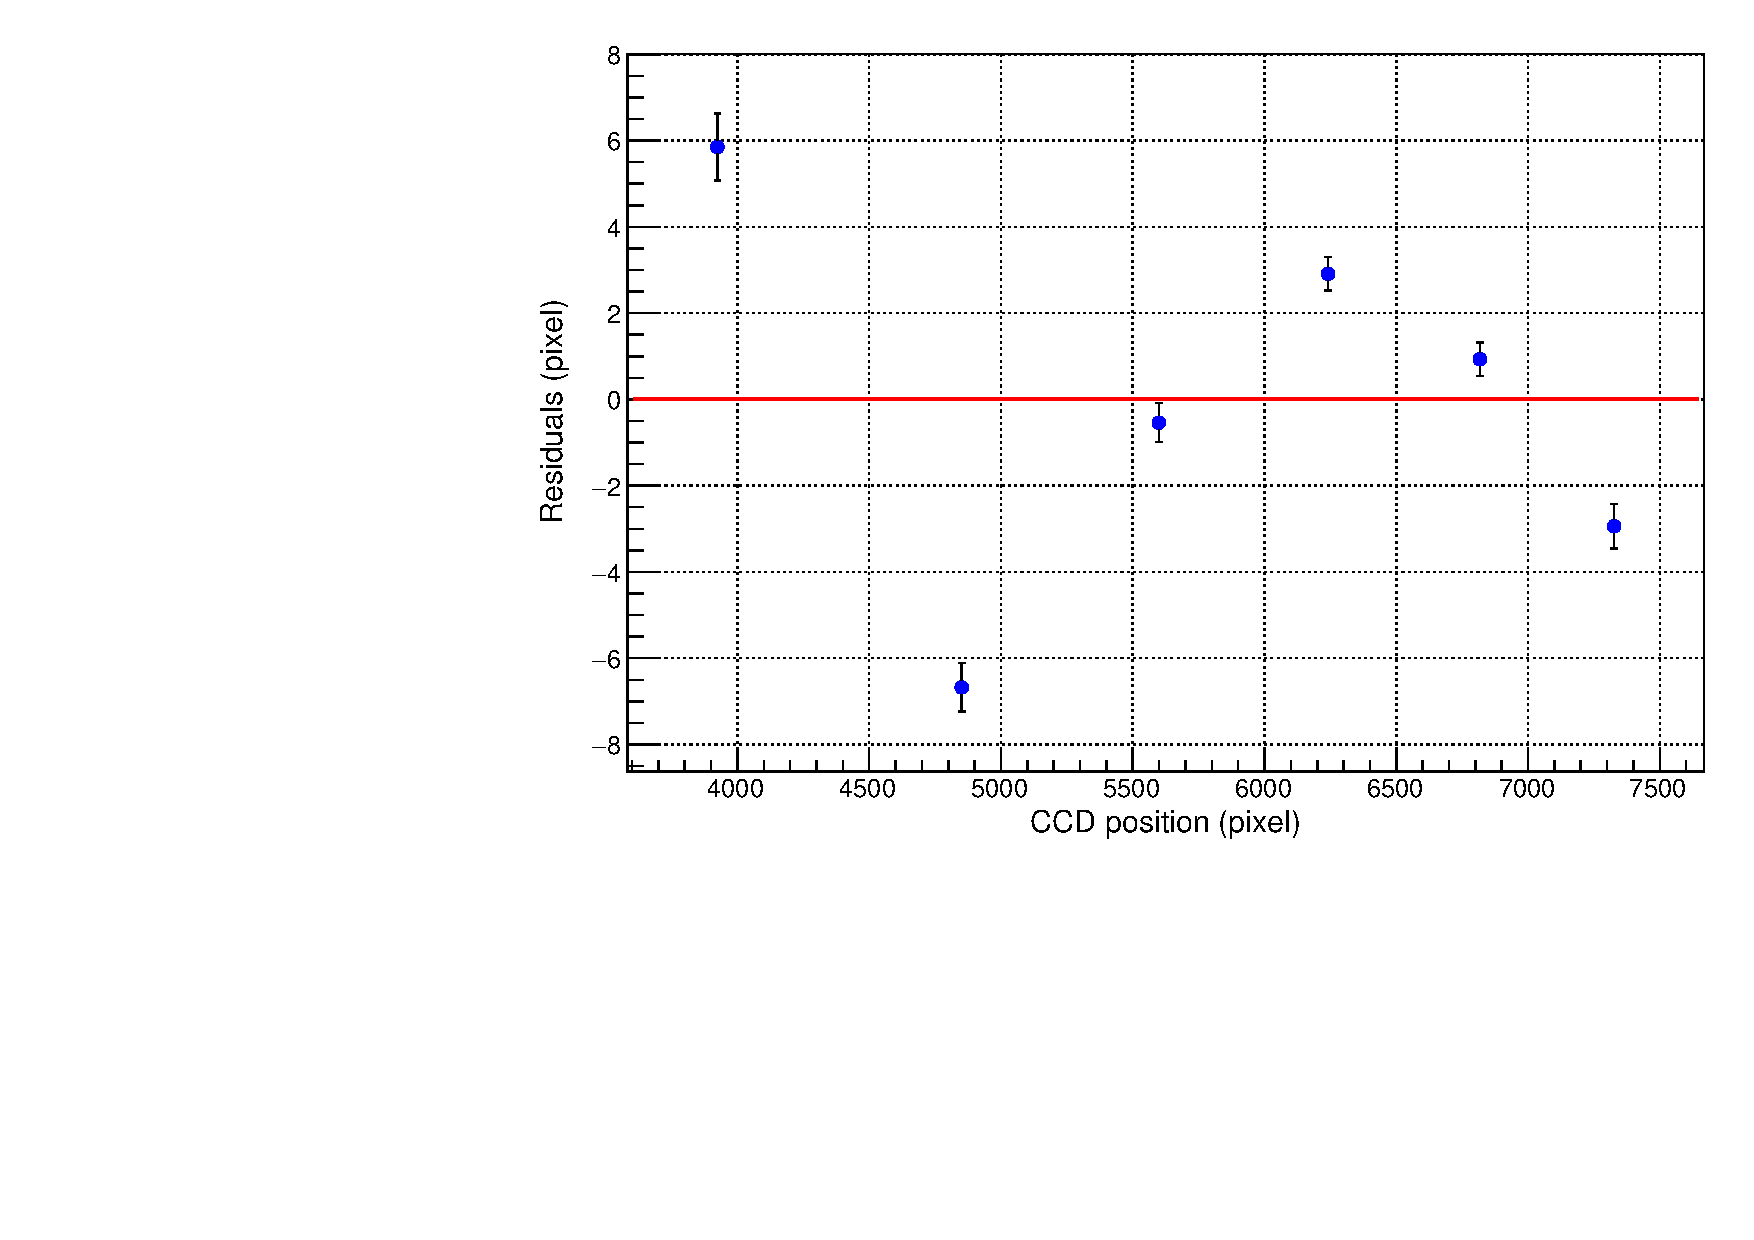
\includegraphics[scale=0.38, angle=0]{campospento/deltaxruBoffres.pdf}
			\setlength{\belowcaptionskip}{-20pt}
			\caption{Andamento dei residui}
			\label{fig:deltaxruBoffres}
		\end{figure}
	\end{center}

	E' evidente che il fit parabolico non può considerarsi ben riuscito: la causa primaria
	può ricercarsi nelle ridotte dimensioni dell'errore responsabili dell'altissimo valore
	di $\chi^{(2)}$, ma è anche da considerare che l'ipotesi quadratica è solamente una 
	prima approssimazione: l'andamento delle spaziature dovrebbe coinvolgere ad esempio 
	anche termini sinusoidali. Il grafico dei residui potrebbe in effetti suggerire tale 
	andamento oscillante.
	

	Si precisa che per calcolare l'errore su tale 
	minimo si è tenuto conto, nella propagazione degli errori, dei termini di 
	covarianza tra i parametri del fit parabolico.
	
	Successivamente si applica la relazione

	\begin{equation}
		\sin(2i) = - \frac{\lambda \sqrt{n^2-1}}{d \Delta i}
	\end{equation}

	da cui si è potuto ottenere una stima dell'angolo i, in particolare

	\[
		i = (1.568 \pm 0.003)\text{rad} = ( 89.8 \pm 0.2 ) ^{\circ}
	\]

	Il valore è compatibile con l'approssimazione a 90°, e inserendolo in \ref{eqn:dlru}
	si otterrà la miglior stima del range di lunghezza d'onda efficace usata
	nel calcolo dei fattori di calibrazione.

	In particolare si è ottenuto

	\[
		\Delta\lambda_{ru} = (0.04353 \pm 0.00008) nm 
	\]	


	\paragraph{Calcolo della risoluzione}

	Il campo magnetico che è possibile sviluppare con l'apparato sperimentale
	arriva fino a un massimo di circa 0.5 T, che genera uno splitting
	di energia di circa $\Delta E_{Zee} = \mu_B B \approx 3\cdot 10^{-5}$ eV.
	Tale separazione corrisponde a una variazione della lunghezza d'onda
	pari a $\Delta \lambda_{Zee} \approx 8 \cdot 10^{-3}$ nm. Sapendo che 
	si è scelto di disporre l'esperimento oscurando la linea di transizione
	centrale, allora per vedere bene lo spitting ci occorrerà una risoluzione
	di almeno

	\[
		R_{th}(\lambda) = \frac{\lambda}{2\Delta\lambda_{Zee}}	\approx 36000
	\]
	Per calcolare la risoluzione effettiva dell'apparato sperimentale
	calcoleremo il rapporto R = $\lambda$ / $\Delta\lambda$ dove 
	$\Delta\lambda$ è dato dalla FWHM dei fit gaussiani effettuati sui 
	picchi. In particolare la FWHM è stata convertita utilizzando la 
	larghezza del pixel in nm, corrispondente a 0.6875$\cdot 10^{-6}$ m.
	Eseguendo dunque i vari rapporti per ciascun fit e calcolando infine
	la media pesata si ottiene

	\[
		R_{sper} = 49015 \pm 637	\quad > R_{th}	
	\]
	che è quindi ben compatibile con la richiesta di minima risoluzione
	necessaria per vedere lo splitting Zeeman con campi magnetici a questo 
	ordine di grandezza.

	Riportiamo in grafico le risoluzioni.

	\begin{center}
		\begin{figure}[H]
			\centering
			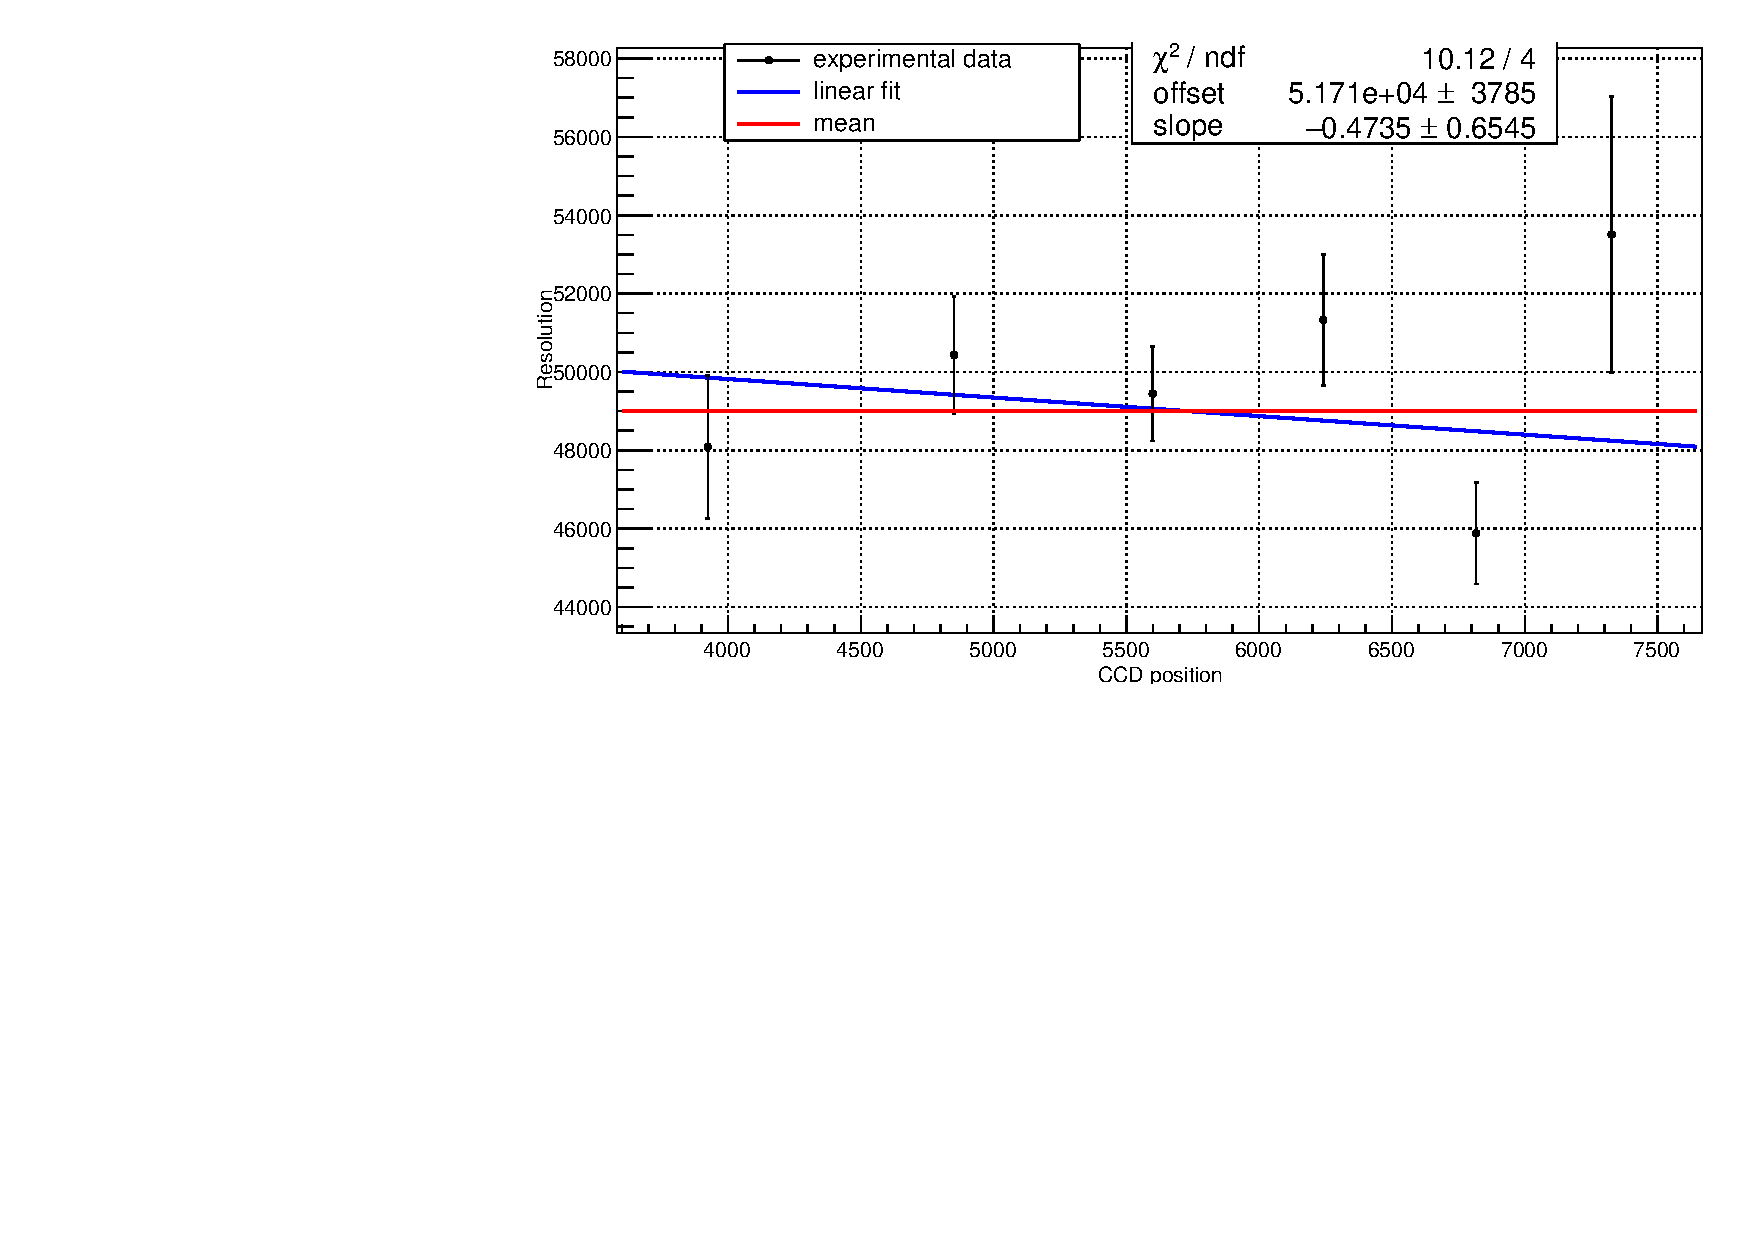
\includegraphics[scale=0.38, angle=0]{campospento/ris.pdf}
			\setlength{\belowcaptionskip}{-20pt}
			\caption{Andamento delle risoluzioni rispetto alla posizione sul CCD}
			\label{fig:deltaxruBoffris}
		\end{figure}
	\end{center}

	\begin{center}
		\begin{figure}[H]
			\centering
			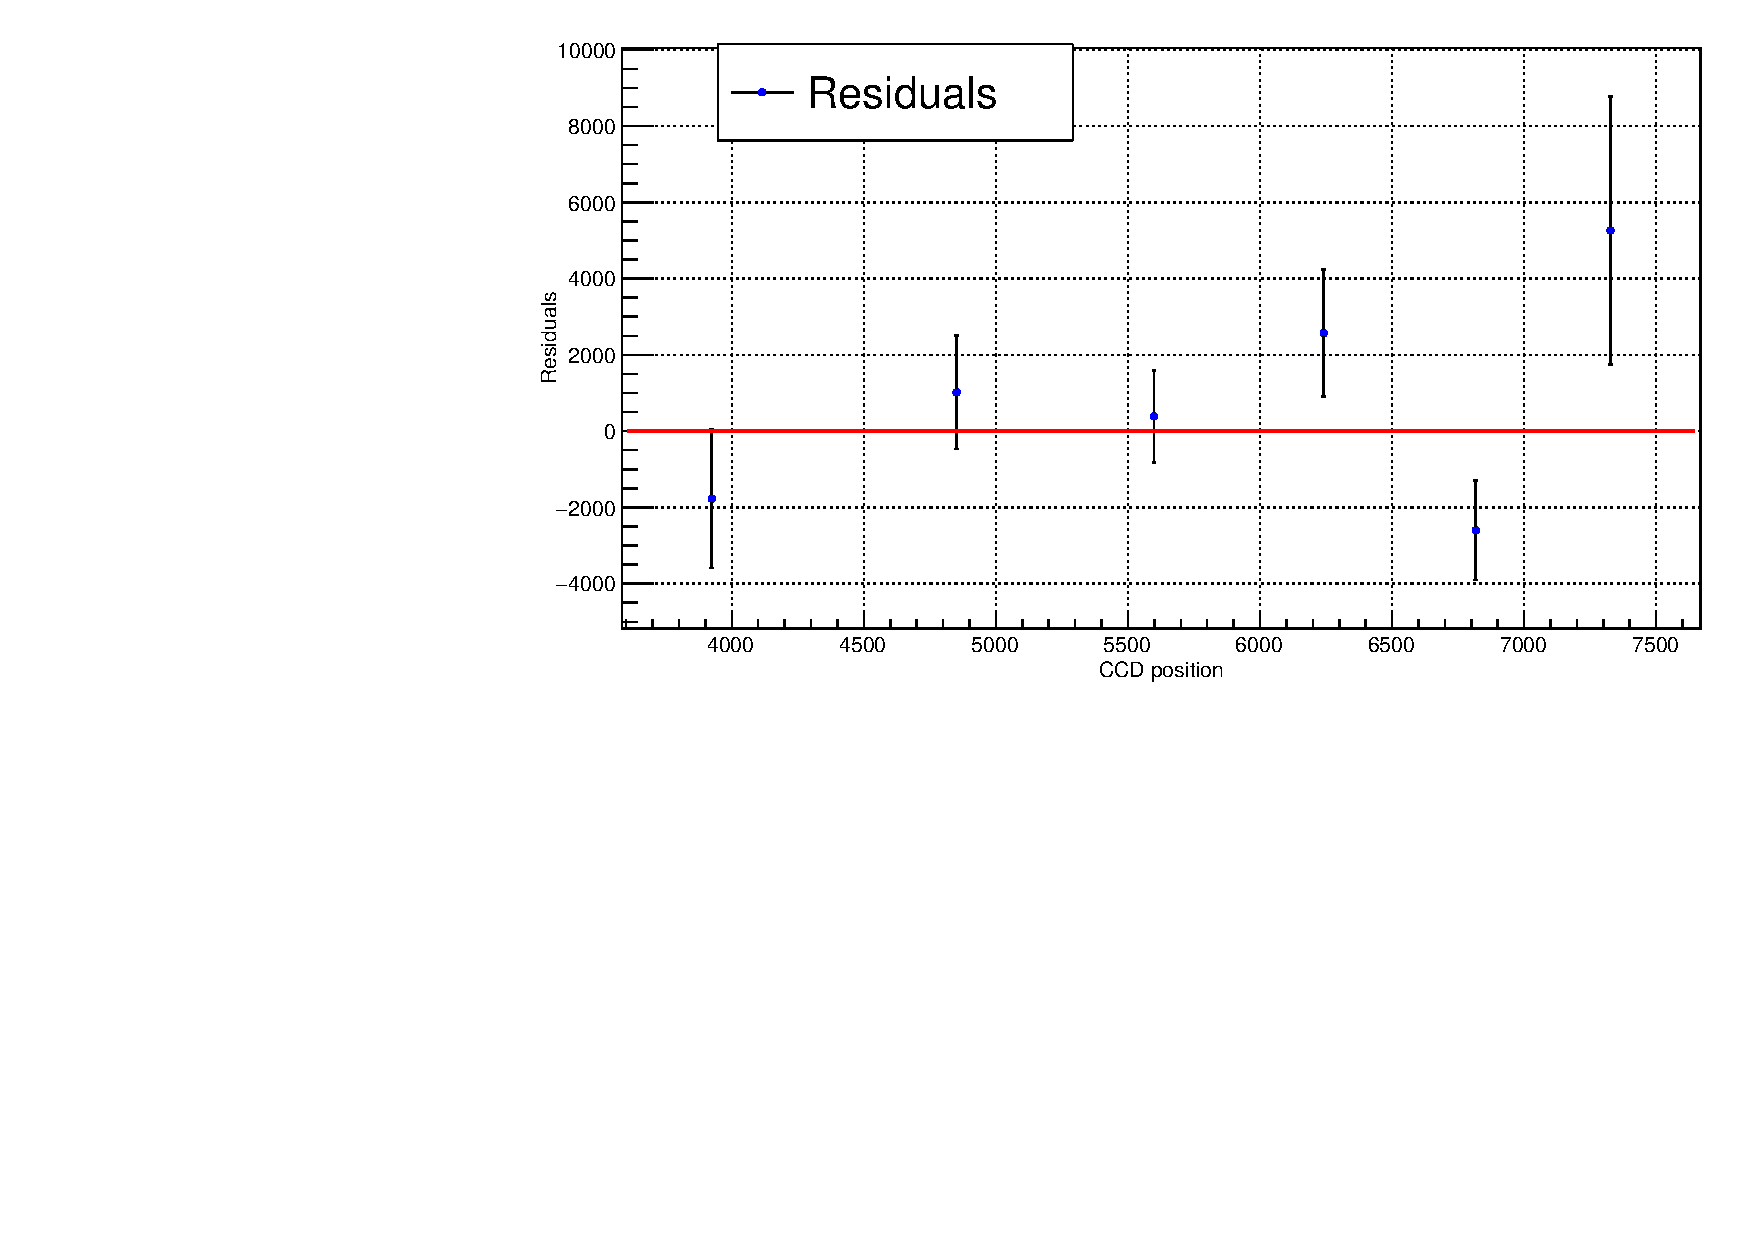
\includegraphics[scale=0.38, angle=0]{campospento/resris.pdf}
			\setlength{\belowcaptionskip}{-20pt}
			\caption{Andamento dei residui}
			\label{fig:deltaxruBoffresris}
		\end{figure}
	\end{center}

	Il fit sulle risoluzioni presenta una compatibilità di $\chi^{(2)}$ data
	da $\lambda \approx$ 2, per cui il fit si può considerare buono, e il valore
	della pendenza è compatibile con lo zero entro 1$\sigma$. Questo autorizza il calcolo della media 
	pesata presentata sopra.


	\subsection*{Campo magnetico acceso}
	
	Si è proceduto quindi accendendo il campo magnetico: inizialmente si è impostato il valore massimo 
	consentito regolando la corrente in modo da ottenere B= 4950 Gauss. 
	Dopodichè si è eseguita nuovamente una calibrazione della posizione della sorgente, ripetendo i 
	passaggi elencati in precedenza, necessaria poichè la presenza del campo magnetico 
	comporta uno shift dello spettro.

	Si è quindi proceduto con l'acquisizione dello spettro inserendo la lamina, ruotando il CCD 
	in verticale, selezionando con i cursori il range e avviando lo scanning, dopo aver un tempo 
	di integrazione pari a 600 ms.
	
	Si ripete quindi  la stessa procedura dopo aver modificato il valore della corrente in modo 
	che il campo magnetico abbia un'intensità circa dimezzata rispetto al valore precedente 
	(B= 2610 Gauss).
	
	\subsubsection*{Campo magnetico massimo}

	Si procede quindi con l'analisi dello spettro.
	In particolare, come anticipato nel compendio teorico, ci si aspetta che ogni picco subisca uno 
	splitting dando luogo a due nuove campane, la cui distanza tra i picchi è indicata con 
	$\Delta \lambda_{Zee} $ .
	 
	Come prima cosa si ripete la procedura di sottrazione del fondo e di rebin della proiezione 
	dell'istogramma bidimensionale sull'asse y, si ottiene quindi lo spettro.
	 
	Dunque si individua il range (in pixel) scelto per l'analisi a campo spento e si suddivide 
	nuovamente in sei gruppi, questa volta ciascun gruppo contiene a sua volta sei campane e 
	non tre a causa dell'effetto Zeeman.
	
	Si è scelto di fittare ciascuna coppia di picchi con una somma di gaussiane, come 
	si vede nel seguente grafico:
	
	\begin{center}
		\begin{figure}[H]
			\centering
			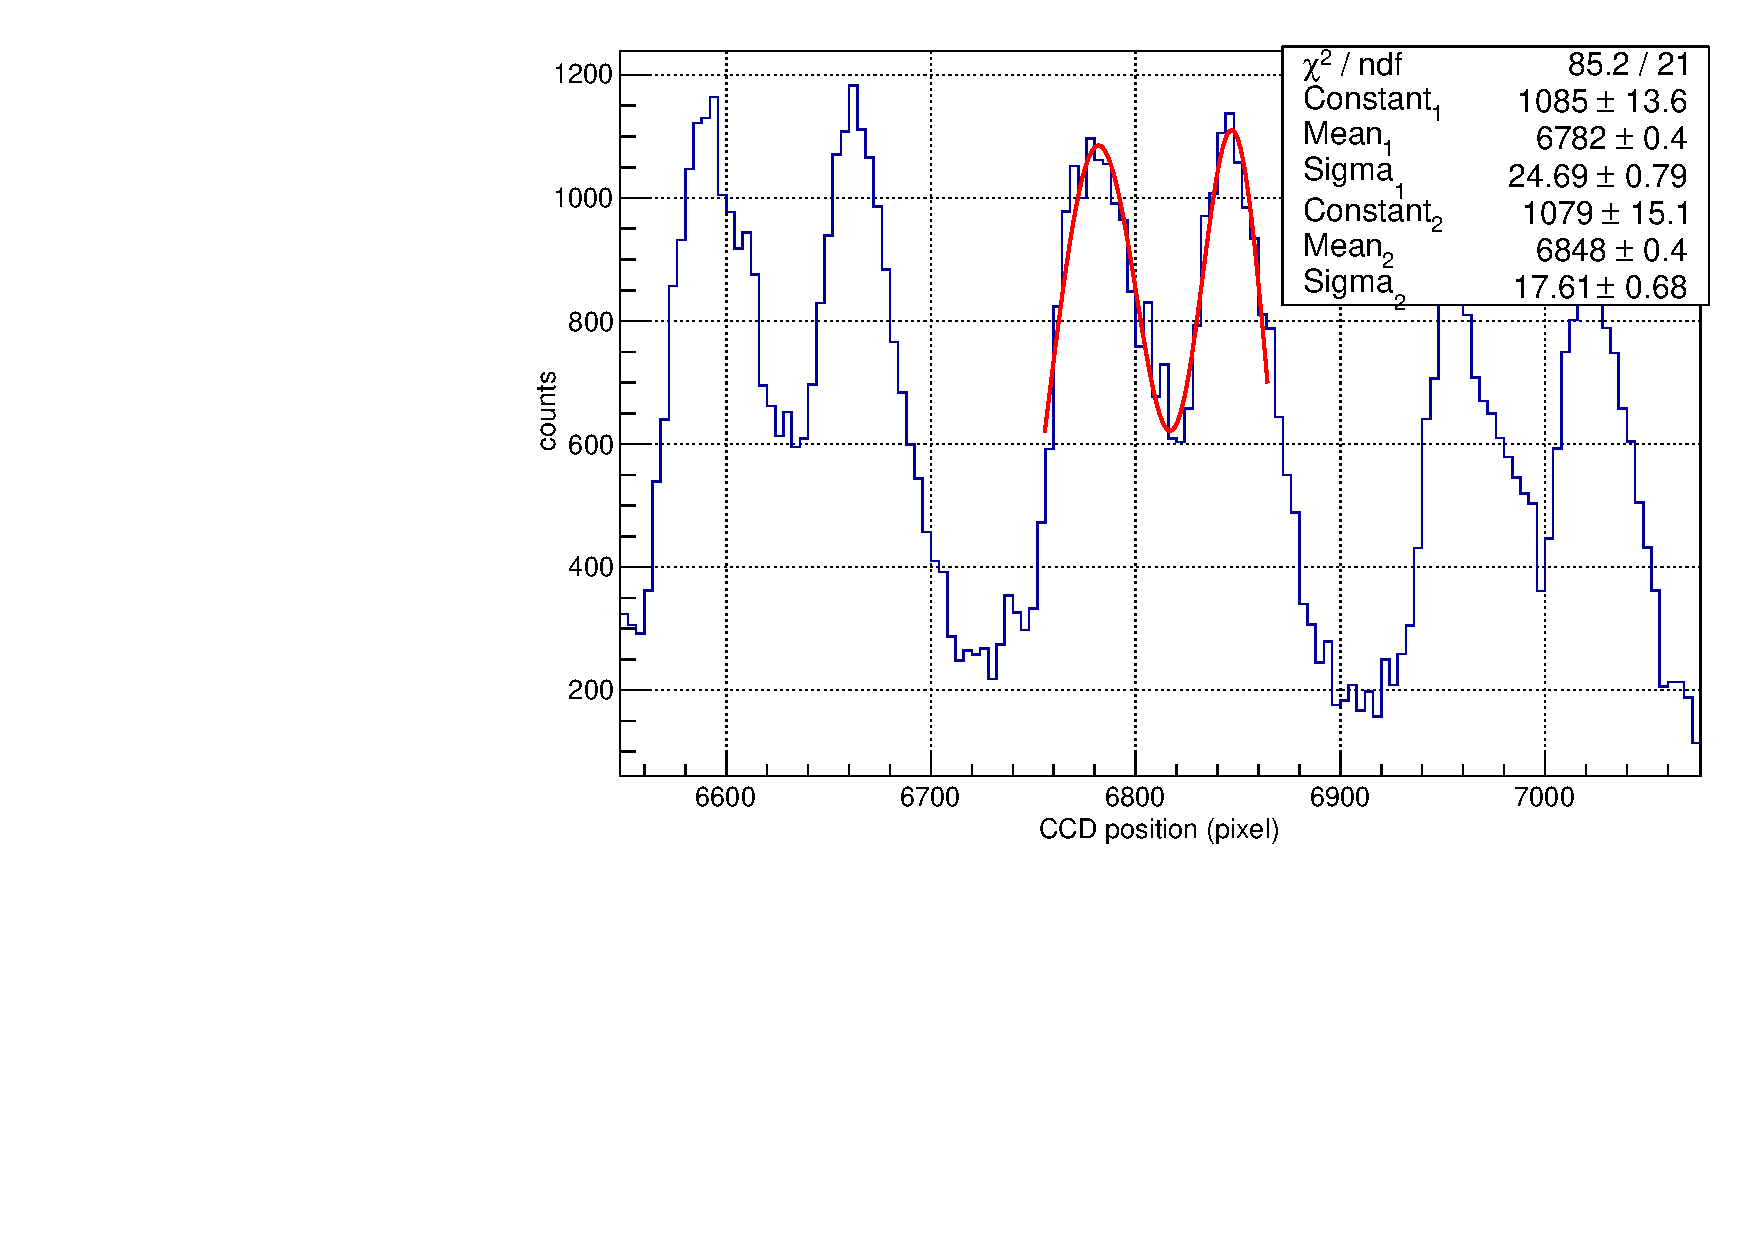
\includegraphics[scale=0.38, angle=0]{campomax/singolo.pdf}
			\setlength{\belowcaptionskip}{-20pt}
			\caption{ Esempio di fit gaussiano nel caso con campo magnetico B= 4950 Gauss}
			\label{fig:singoloBonMax}
		\end{figure}
	\end{center}

	Anche in questo caso il valore di $\chi^{(2)}$ risulta incompatibile con il suo
	valore di aspettazione ($\lambda \approx 9.9$). Come detto in precedenza, la scelta
	del range risulta determinante sul valore del $\chi^{(2)}$, per cui sarebbe forse
	stato più conveniente da questo punto di vista scegliere di fittare in modo indipendente
	i due picchi ciascuno con una gaussiana, piuttosto che usare la somma delle due che 
	limita la libertà di regolazione del range. Tuttavia si è fatta questa scelta per coerenza
	con il processo di acquisizione dei dati. Infatti dal momento che i dati si distribuiscono
	con una certa dispersione attorno ai picchi, allora ognuna delle code esercita un'influenza
	sul picco dell'altra distribuzione.


	Ripetuto questo tipo di interpolazione per le coppie di picchi splittati, si è calcolata di volta 
	in volta la distanza in pixel $\Delta x_{Zee}$ come la differenza tra le ascisse dei centri delle due
	gaussiane. Tale differenza corrisponde in realtà a due volte lo splitting fisico, per via della 
	configurazione dell'apparato che sopprime la riga centrale.

	Riportiamo di seguito un plot dei rapporti $\Delta x_{Zee}$/$\Delta x_{ru}$, usando le $\Delta x_{ru}$
	calcolate nel caso a campo spento, rispetto alla posizione sul CCD: vediamo come tale quantità resti 
	costante.

	\begin{center}
		\begin{figure}[H]
			\centering
			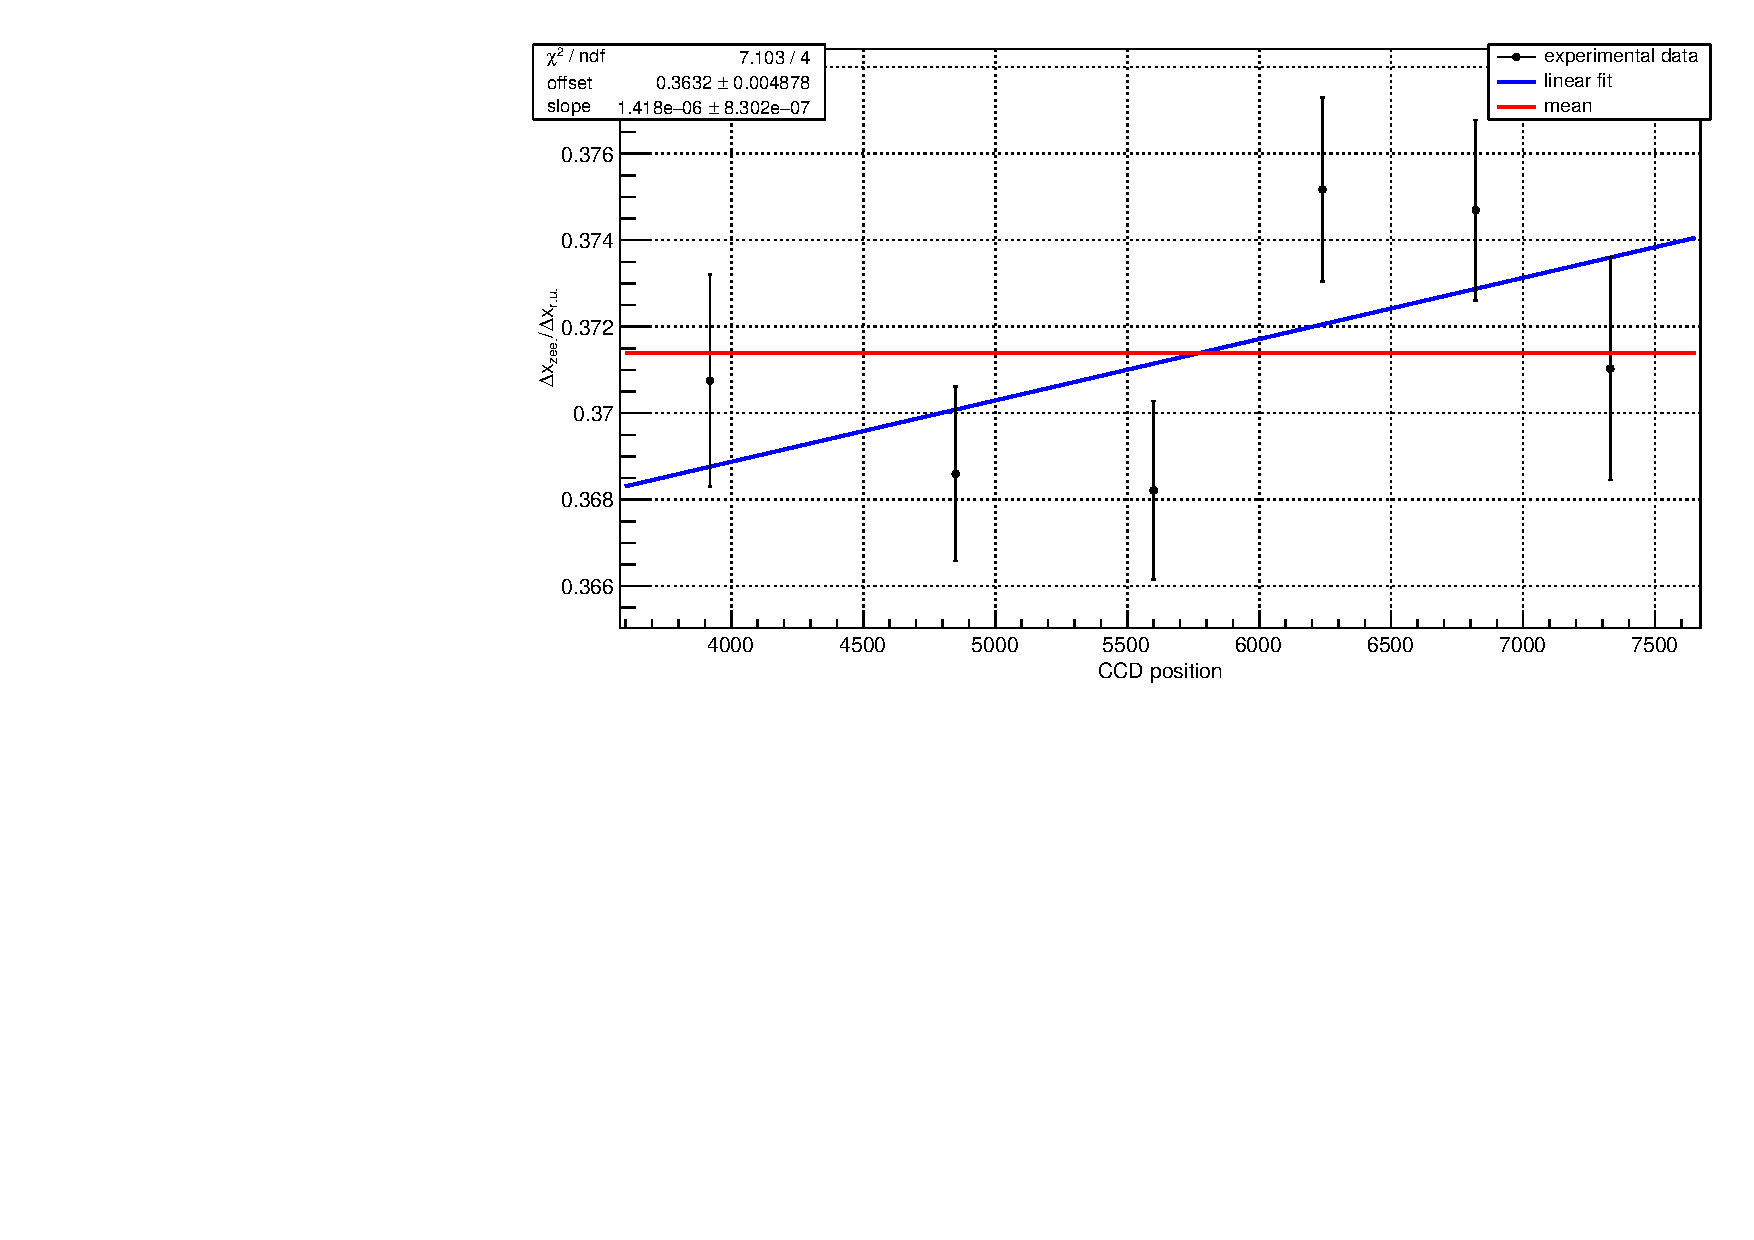
\includegraphics[scale=0.38, angle=0]{campomax/fit.pdf}
			\setlength{\belowcaptionskip}{-20pt}
			\caption{Andamento del rapporto $\Delta x_{Zee}$/$\Delta x_{ru}$}
			\label{fig:fit_rapporto}
		\end{figure}
	\end{center}

	\begin{center}
		\begin{figure}[H]
			\centering
			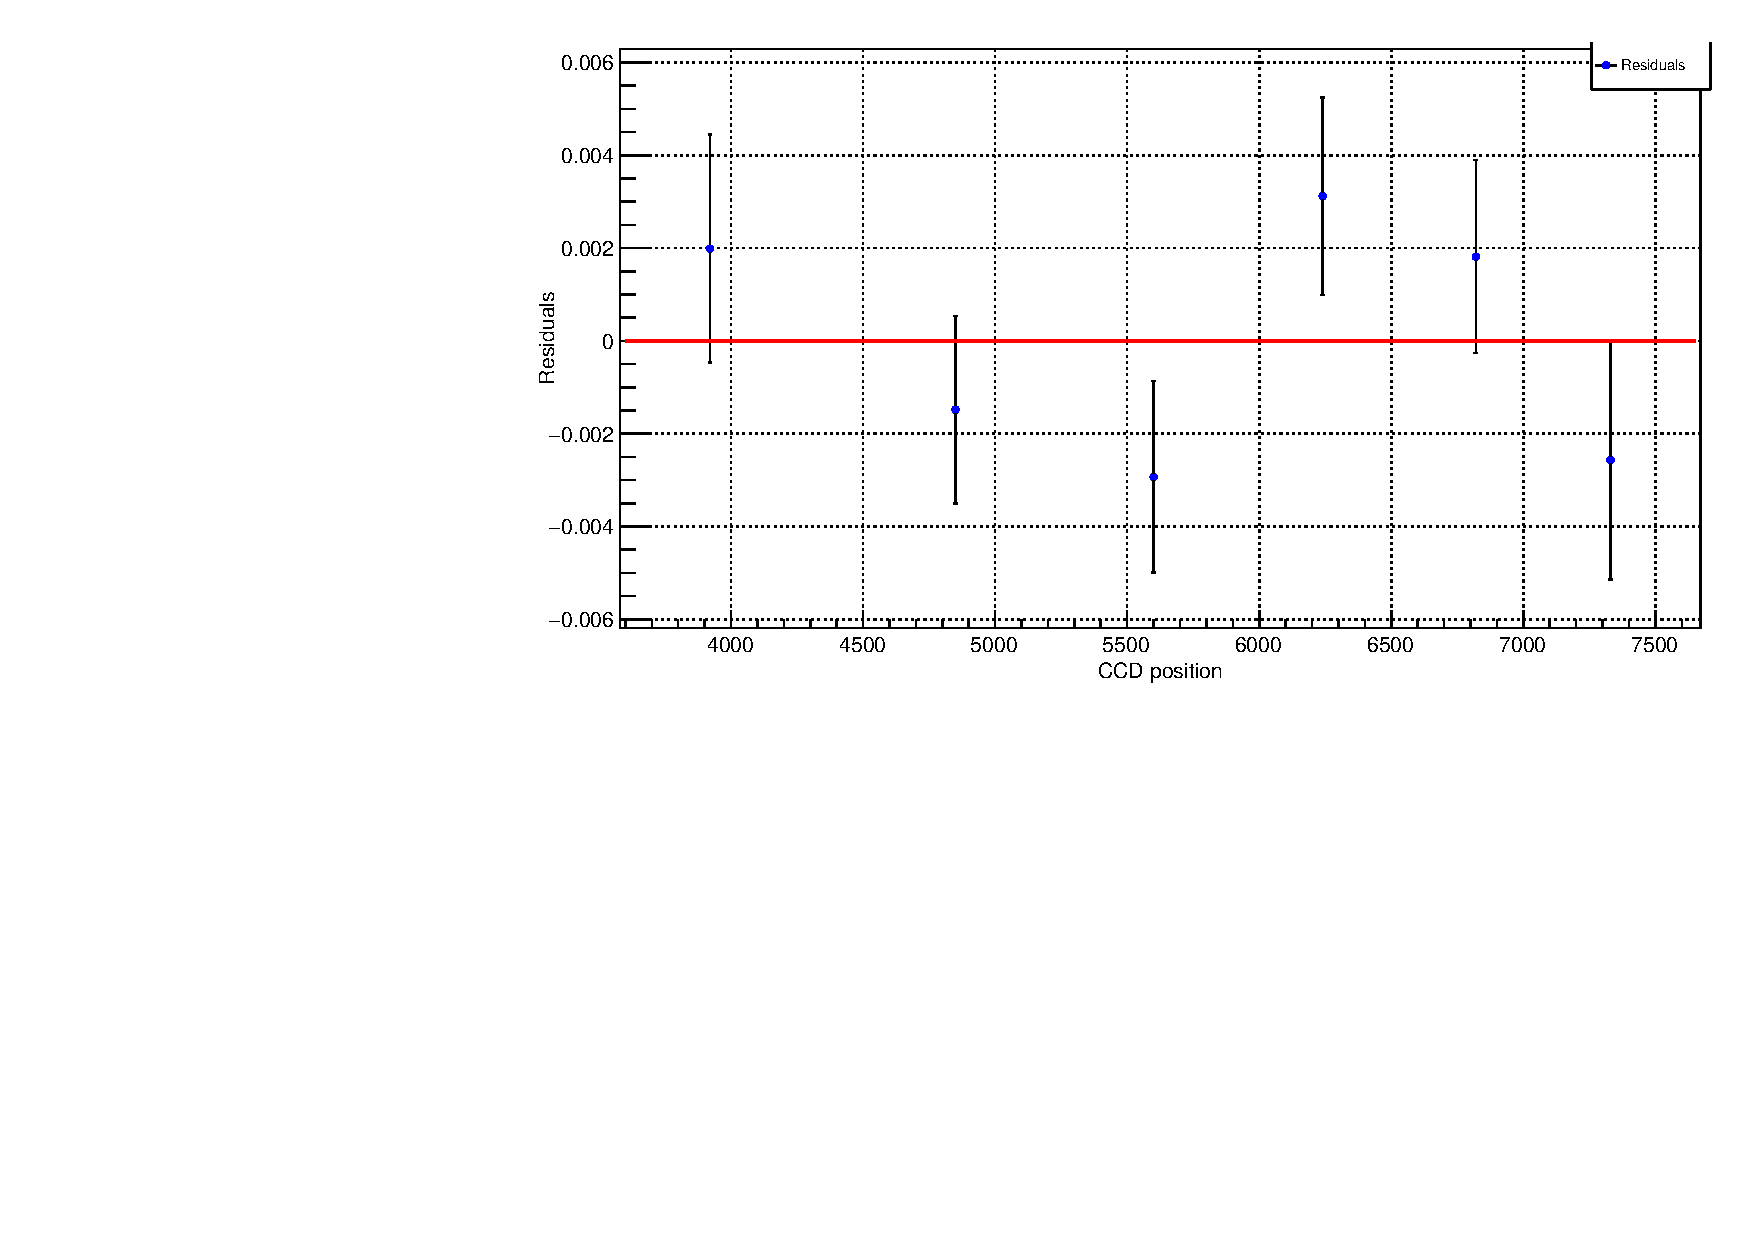
\includegraphics[scale=0.38, angle=0]{campomax/residuals.pdf}
			\setlength{\belowcaptionskip}{-20pt}
			\caption{Andamento dei residui}
			\label{fig:fit_rapporto_res}
		\end{figure}
	\end{center}

	La pendenza della retta con cui si è fittata la distribuzione dei rapporti è effettivamente
	compatibile con lo zero entro 2$\sigma$. Questo autorizza il calcolo della media pesata, per cui 
	la miglior stima del rapporto in questione è data da 

	\[
		\frac{\Delta x_{Zee}}{\Delta x_{ru}} = 0.3714 \pm 0.0009	
	\]
	Mostriamo anche un grafico equivalente con l'andamento di $\Delta\lambda_{Zee}$, ossia 
	$\Delta x_{Zee}$ opportunamente convertito con il fattore F caratteristico della relativa regione
	dello spettro.

	\begin{center}
		\begin{figure}[H]
			\centering
			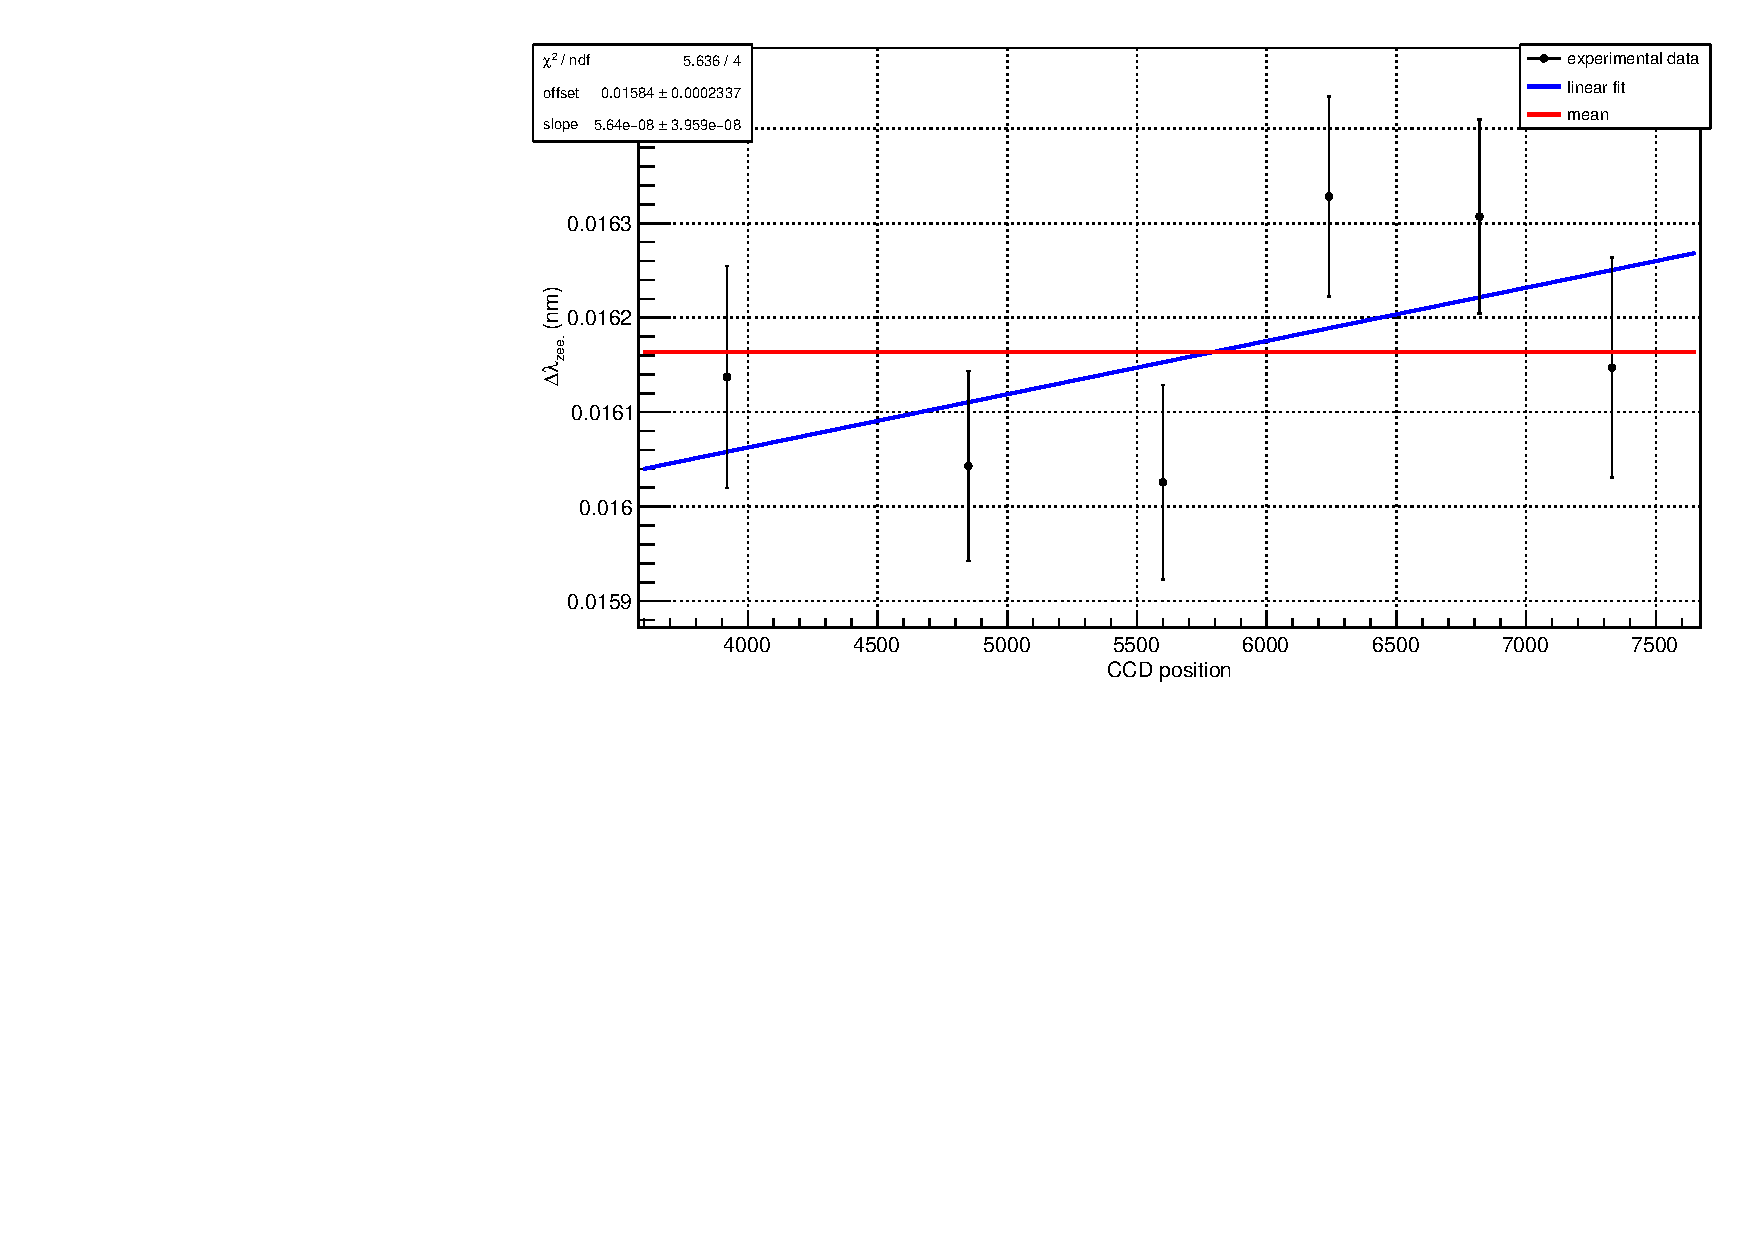
\includegraphics[scale=0.38, angle=0]{campomax/dlambdazee.pdf}
			\setlength{\belowcaptionskip}{-20pt}
			\caption{Andamento dello shifting Zeeman}
			\label{fig:fit_dlambdazee}
		\end{figure}
	\end{center}

	\begin{center}
		\begin{figure}[H]
			\centering
			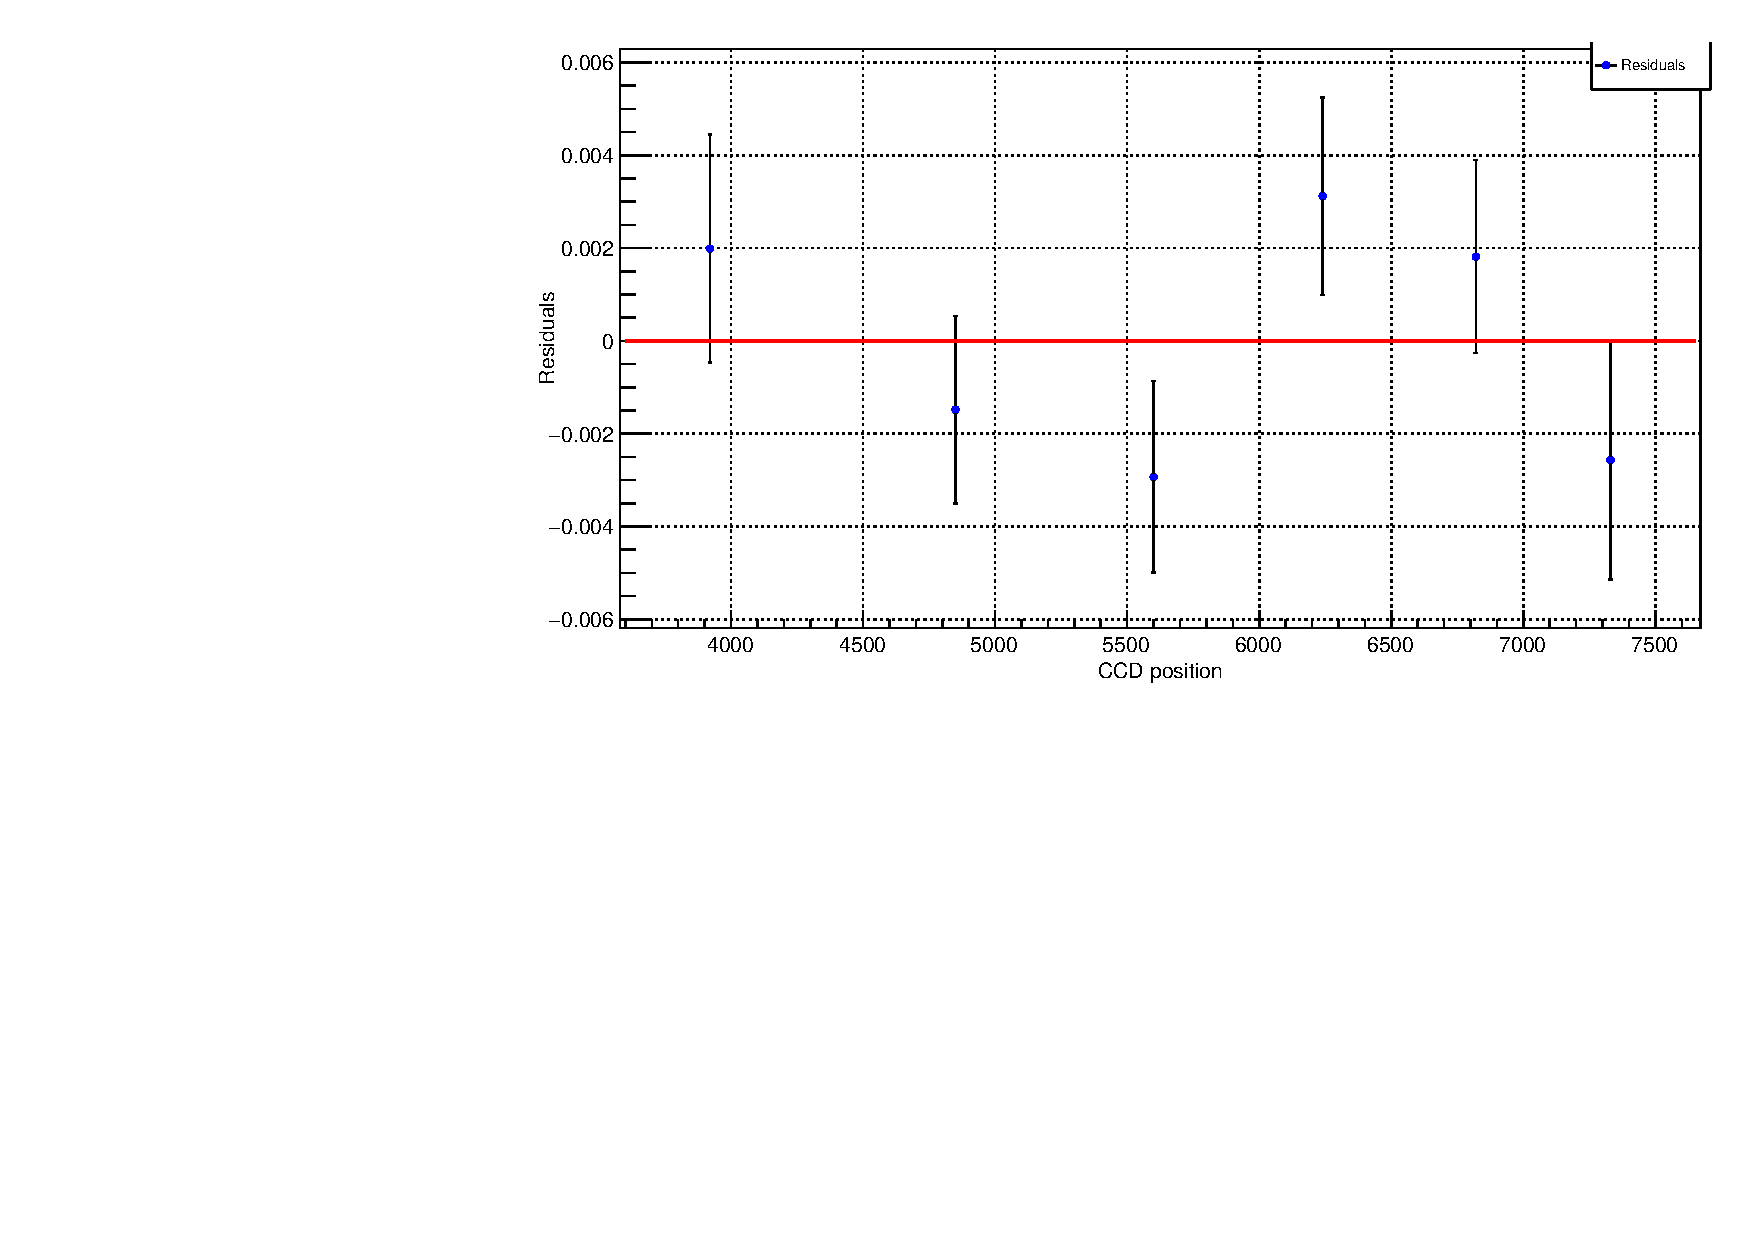
\includegraphics[scale=0.38, angle=0]{campomax/residuals.pdf}
			\setlength{\belowcaptionskip}{-20pt}
			\caption{Andamento dei residui}
			\label{fig:fit_dlambdazee_res}
		\end{figure}
	\end{center}

	Da cui si ricava per media pesata la miglior stima dello shifting Zeeman

	\[
		\Delta\lambda_{Zee} = (1.616 \pm 0.004) \cdot 10^{-2} nm	
	\]

	che corrisponde al valore del rapporto precedentemente fornito moltiplicato per $\Delta\lambda_{ru}$.

	Si dispone dunque di tutti gli elementi per calcolare finalmente il fattore di Landé. In particolare

	\begin{equation}
		\Delta E_{Zee} = g \mu_B B
	\end{equation}

	dove $\mu_B$ è il magnetone di Bohr.
	Dal momento che $\Delta E = h\Delta\nu = hc\Delta(1/\lambda) = (hc / \lambda^2) \Delta\lambda$, 
	allora vale 

	\begin{equation}
		g = \frac{hc}{\mu_B B \lambda^2} \frac{\Delta\lambda_{Zee}}{2}
	\end{equation}

	\begin{center}
		\begin{figure}[H]
			\centering
			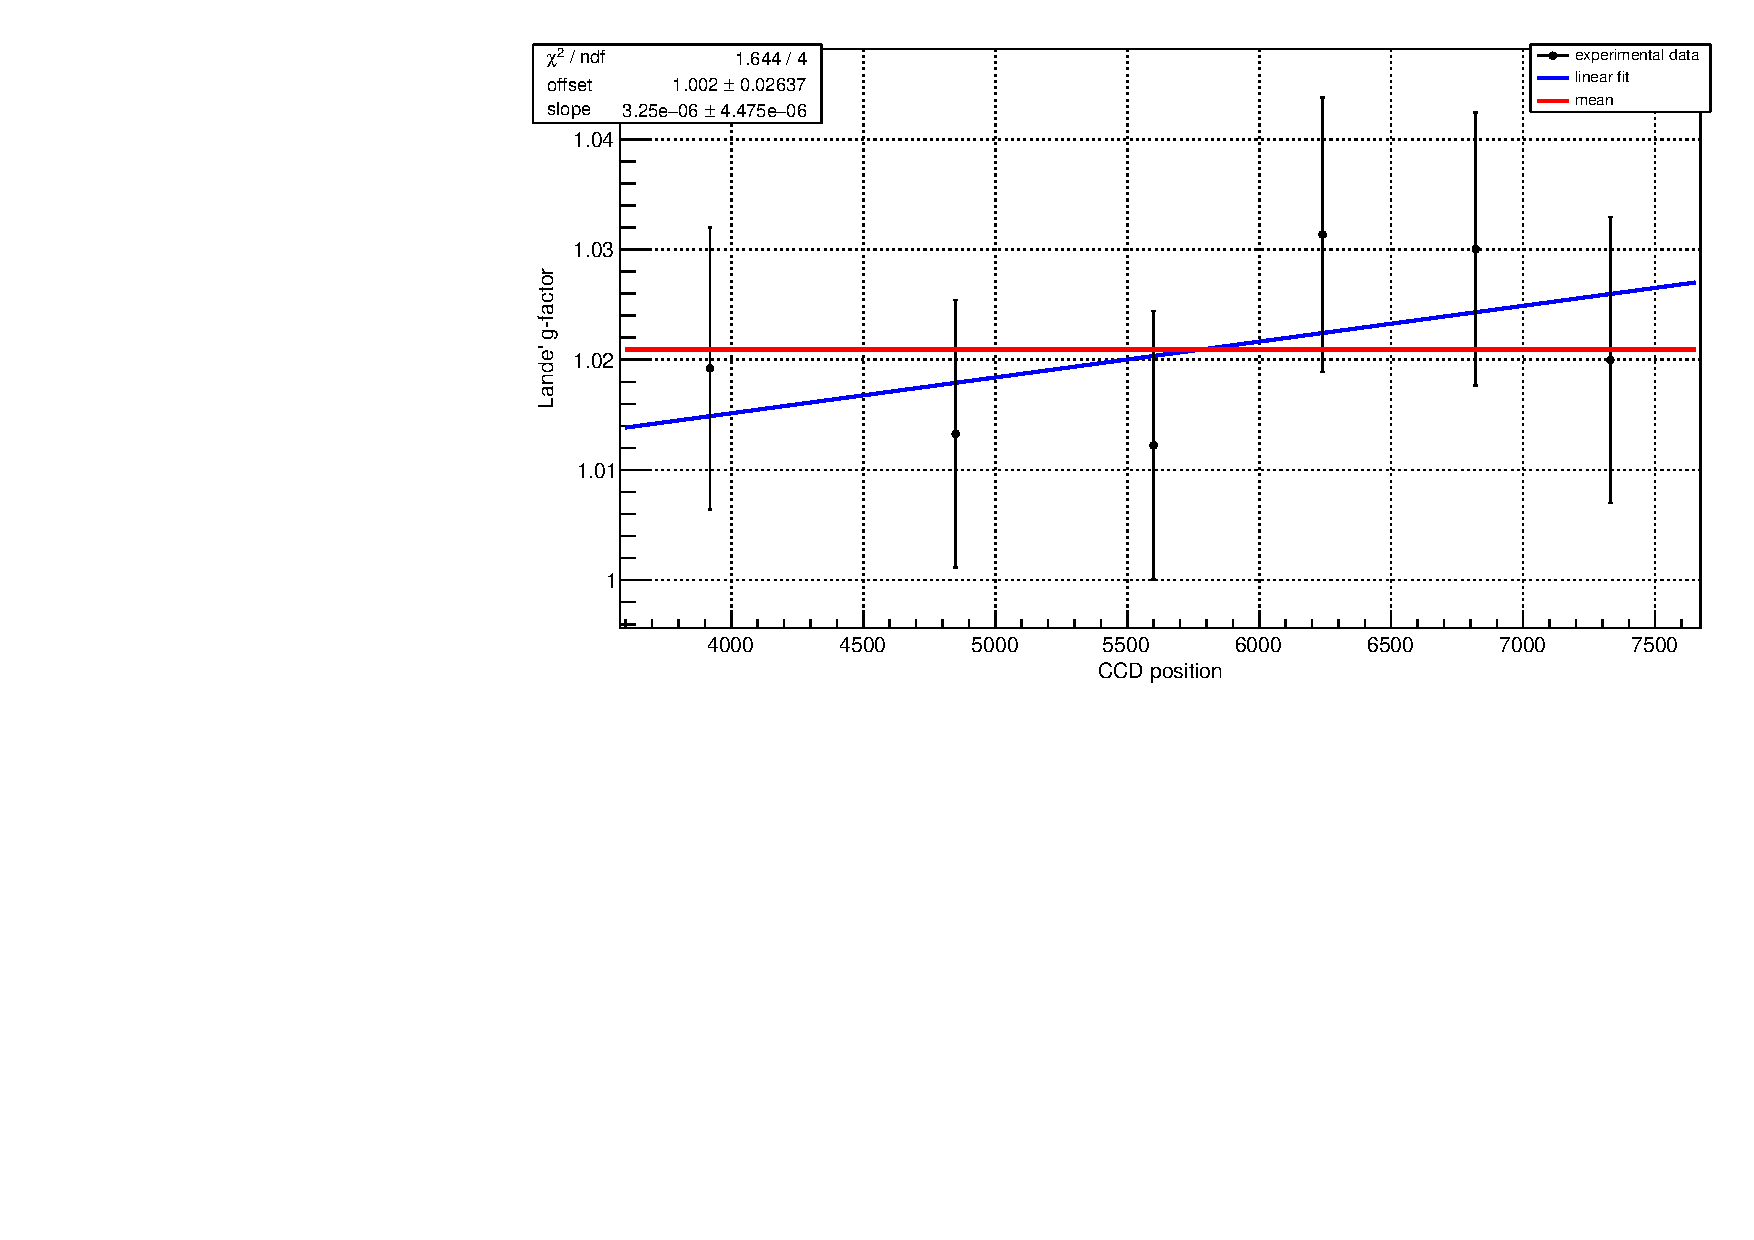
\includegraphics[scale=0.38, angle=0]{campomax/g.pdf}
			\setlength{\belowcaptionskip}{-20pt}
			\caption{Andamento del fattore giromagnetico}
			\label{fig:g}
		\end{figure}
	\end{center}

	\begin{center}
		\begin{figure}[H]
			\centering
			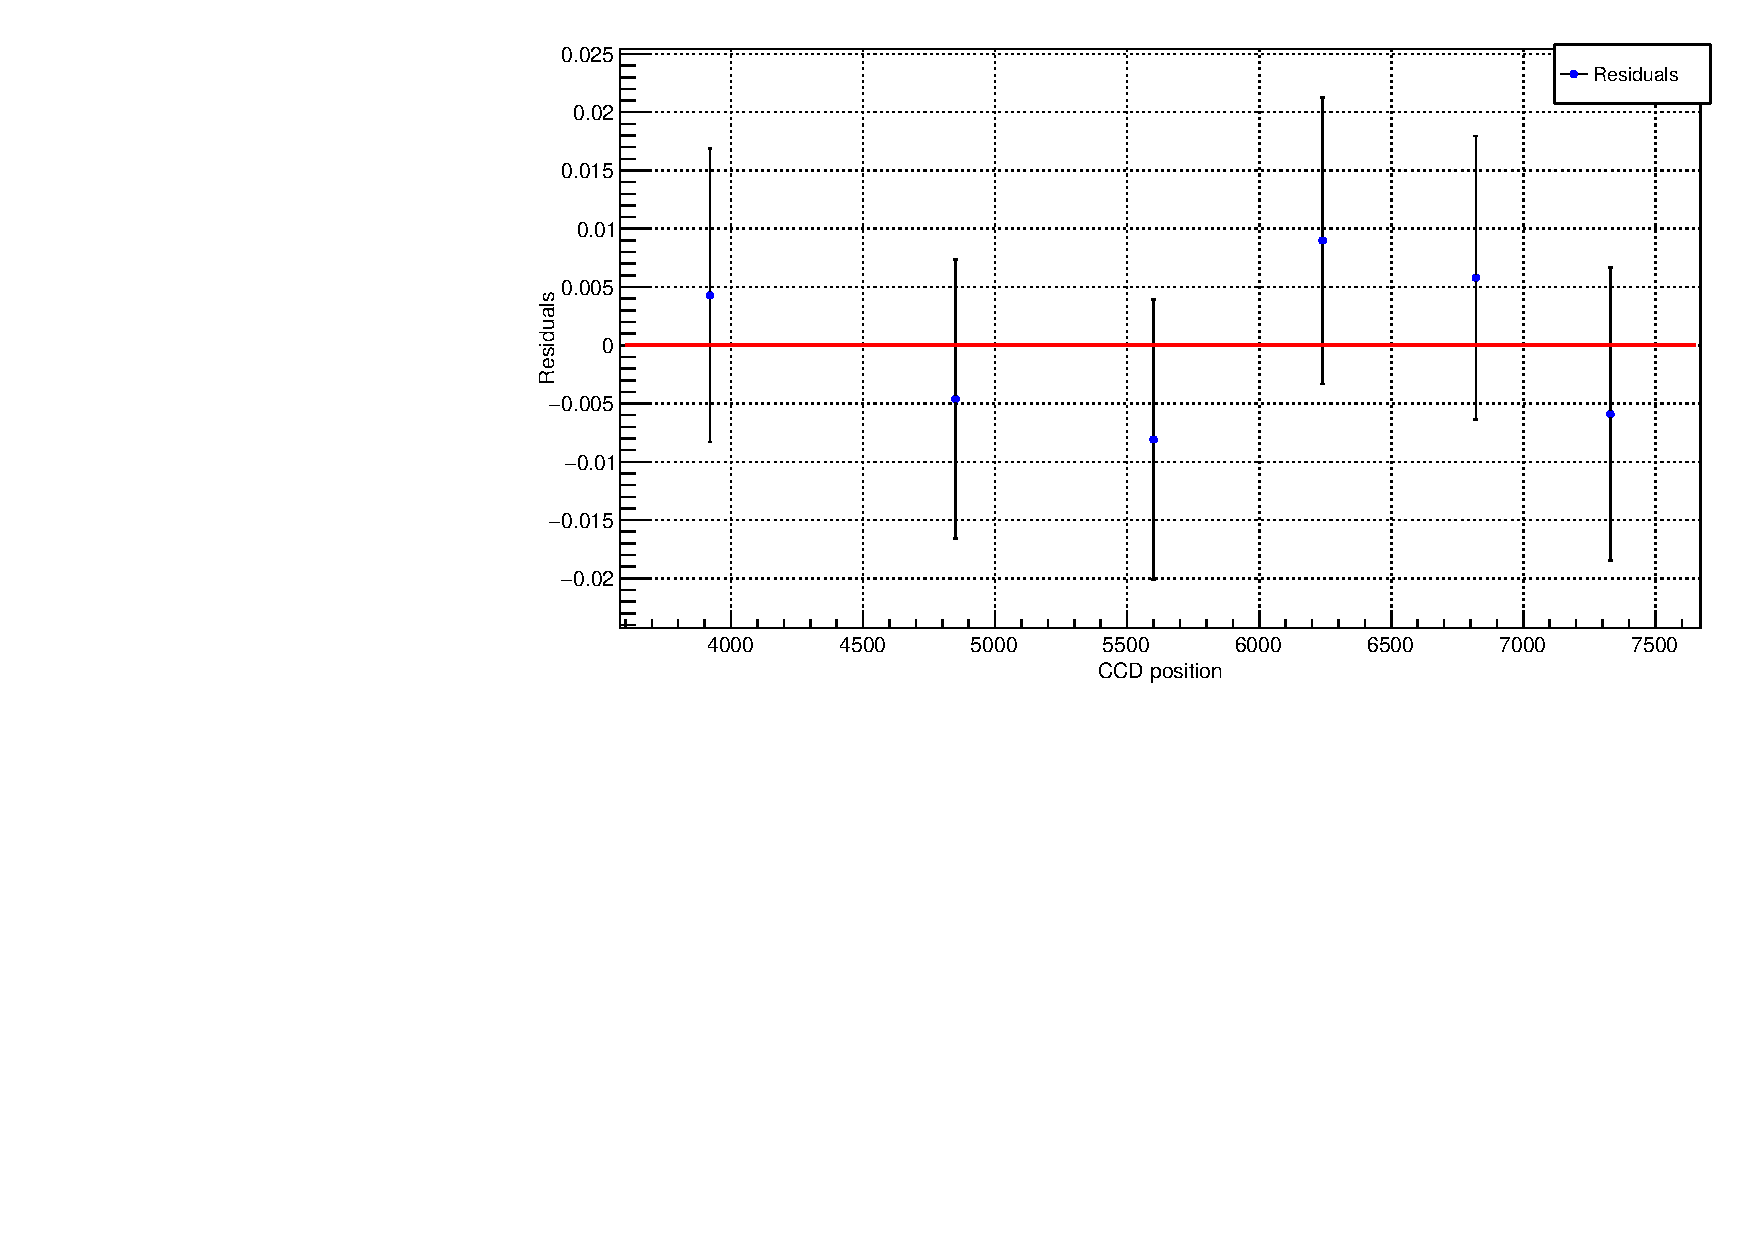
\includegraphics[scale=0.38, angle=0]{campomax/g_residuals.pdf}
			\setlength{\belowcaptionskip}{-20pt}
			\caption{Andamento dei residui}
			\label{fig:g_res}
		\end{figure}
	\end{center}

	Si vede subito che la pendenza del fit lineare è compatibile con lo zero entro 1$\sigma$. 
	
	Si presenta dunque il fattore g ottenuto dal $\Delta\lambda_{zee}$ pesato.

	\[
		g = 1.02 \pm 0.01
	\]
	
	che risulta compatibile con il valore atteso g = 1.
	Lo scarto corrisponde infatti circa a 2$\sigma$.  

	 
	\subsubsection*{Campo magnetico dimezzato}

	Si ripete un'analisi del tutto analogo anche per il caso con campo magnetico di intensità dimezzata.
	
	
	\begin{center}
	\begin{figure}[H]
		\centering
		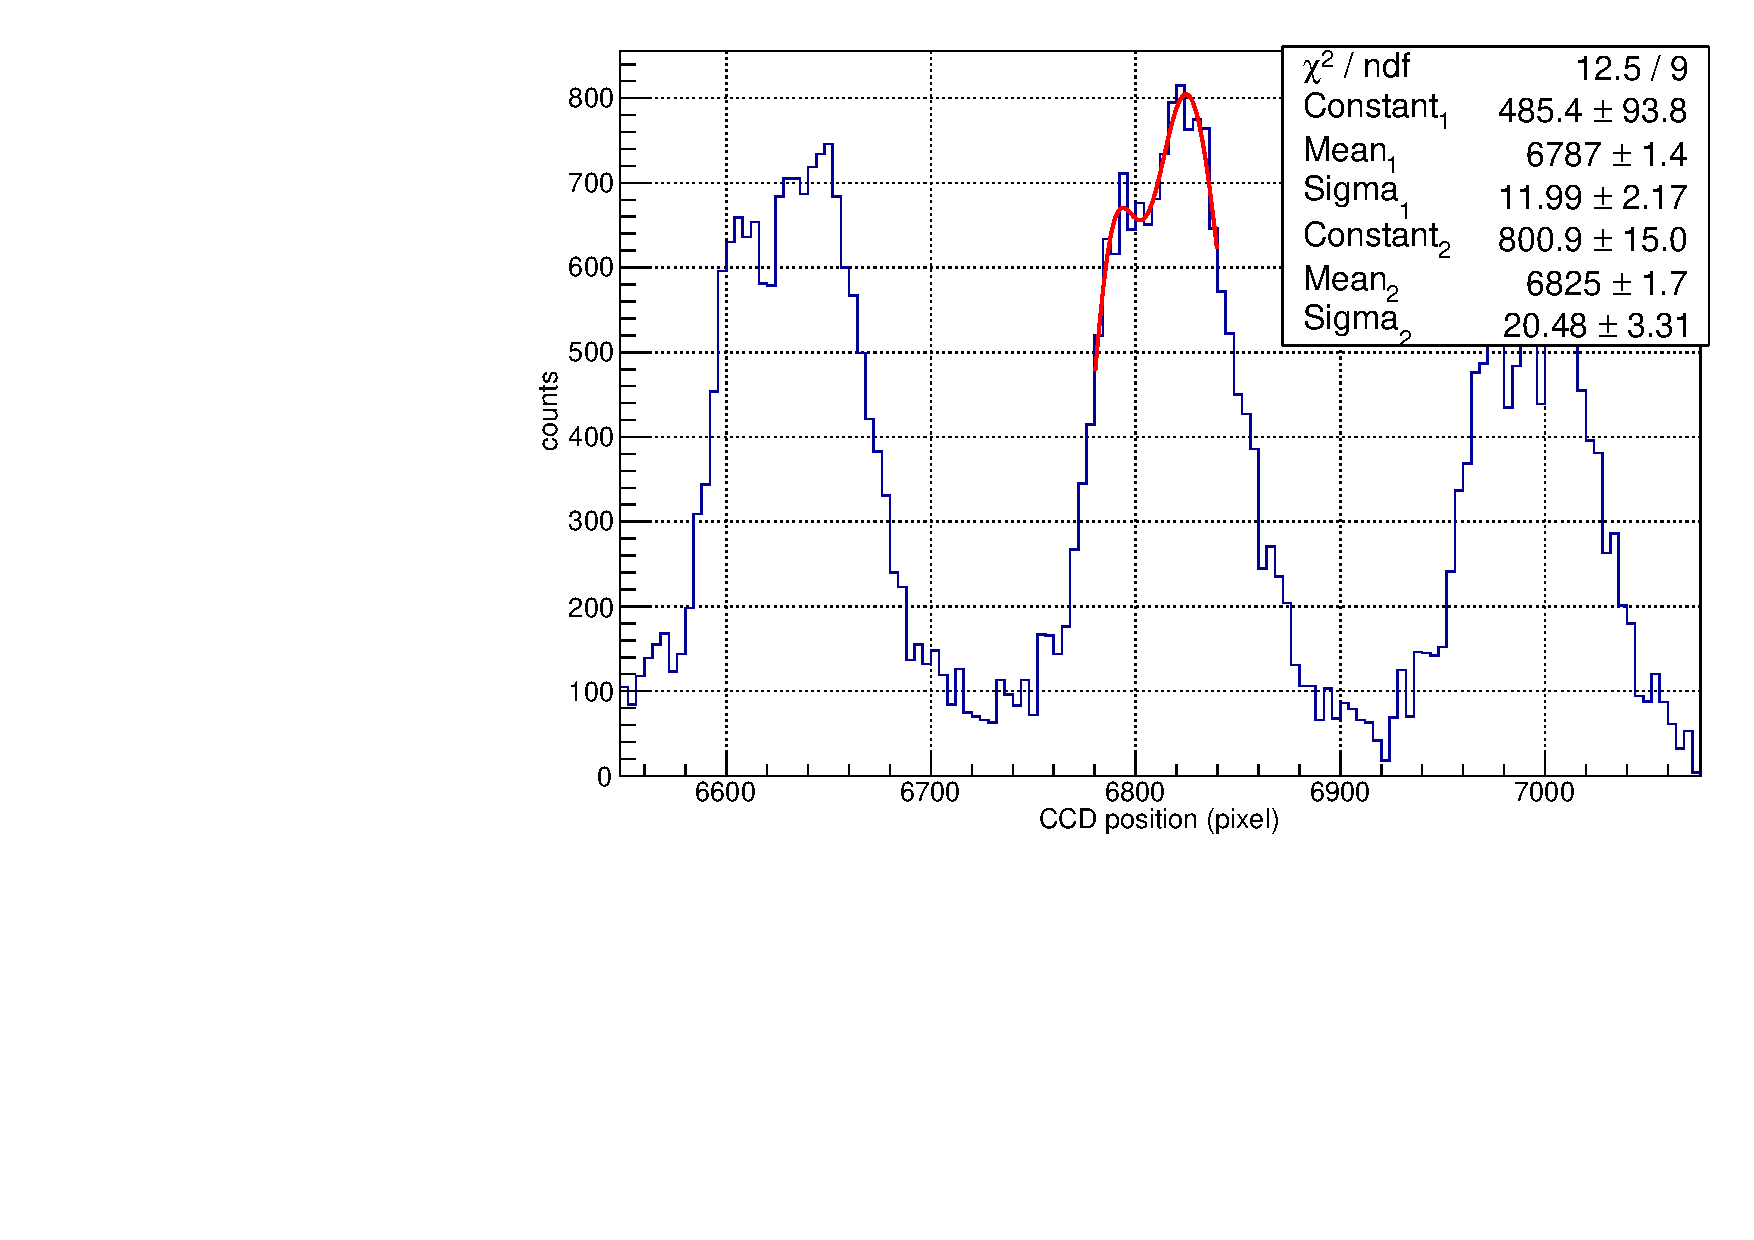
\includegraphics[scale=0.38, angle=0]{campomin/singolo.pdf}
        \setlength{\belowcaptionskip}{-20pt}
		\caption{ Esempio di fit gaussiano nel caso con campo magnetico B= 2610 Gauss}
		\label{fig:singoloBonMin}
	\end{figure}
	\end{center}

	Si osserva che questa situazione corrisponde a uno dei quei casi in cui il valore di
	$\chi^{(2)}$ risulta ottimale ($\lambda\approx 0.8$), nonostante il fit sia stato effettuato
	come somma di due gaussiane.
	Per garantire una buona interpolazione dei dati si è pensato di tenere fissa la $\sigma$
	della campana pari a quella ottenuta a campo massimo, tuttavia dopo alcuni risultati non
	particolarmente positivi, si è preferito inserire i parametri del caso $B_{max}$ come
	dati iniziali riuscendo così a ottenere risultati migliori.
	
	Riportiamo di nuovo un plot dei rapporti $\Delta x_{Zee}$/$\Delta x_{ru}$, usando le $\Delta x_{ru}$
	calcolate nel caso a campo spento, rispetto alla posizione sul CCD: vediamo come tale quantità resti 
	costante.

	\begin{center}
		\begin{figure}[H]
			\centering
			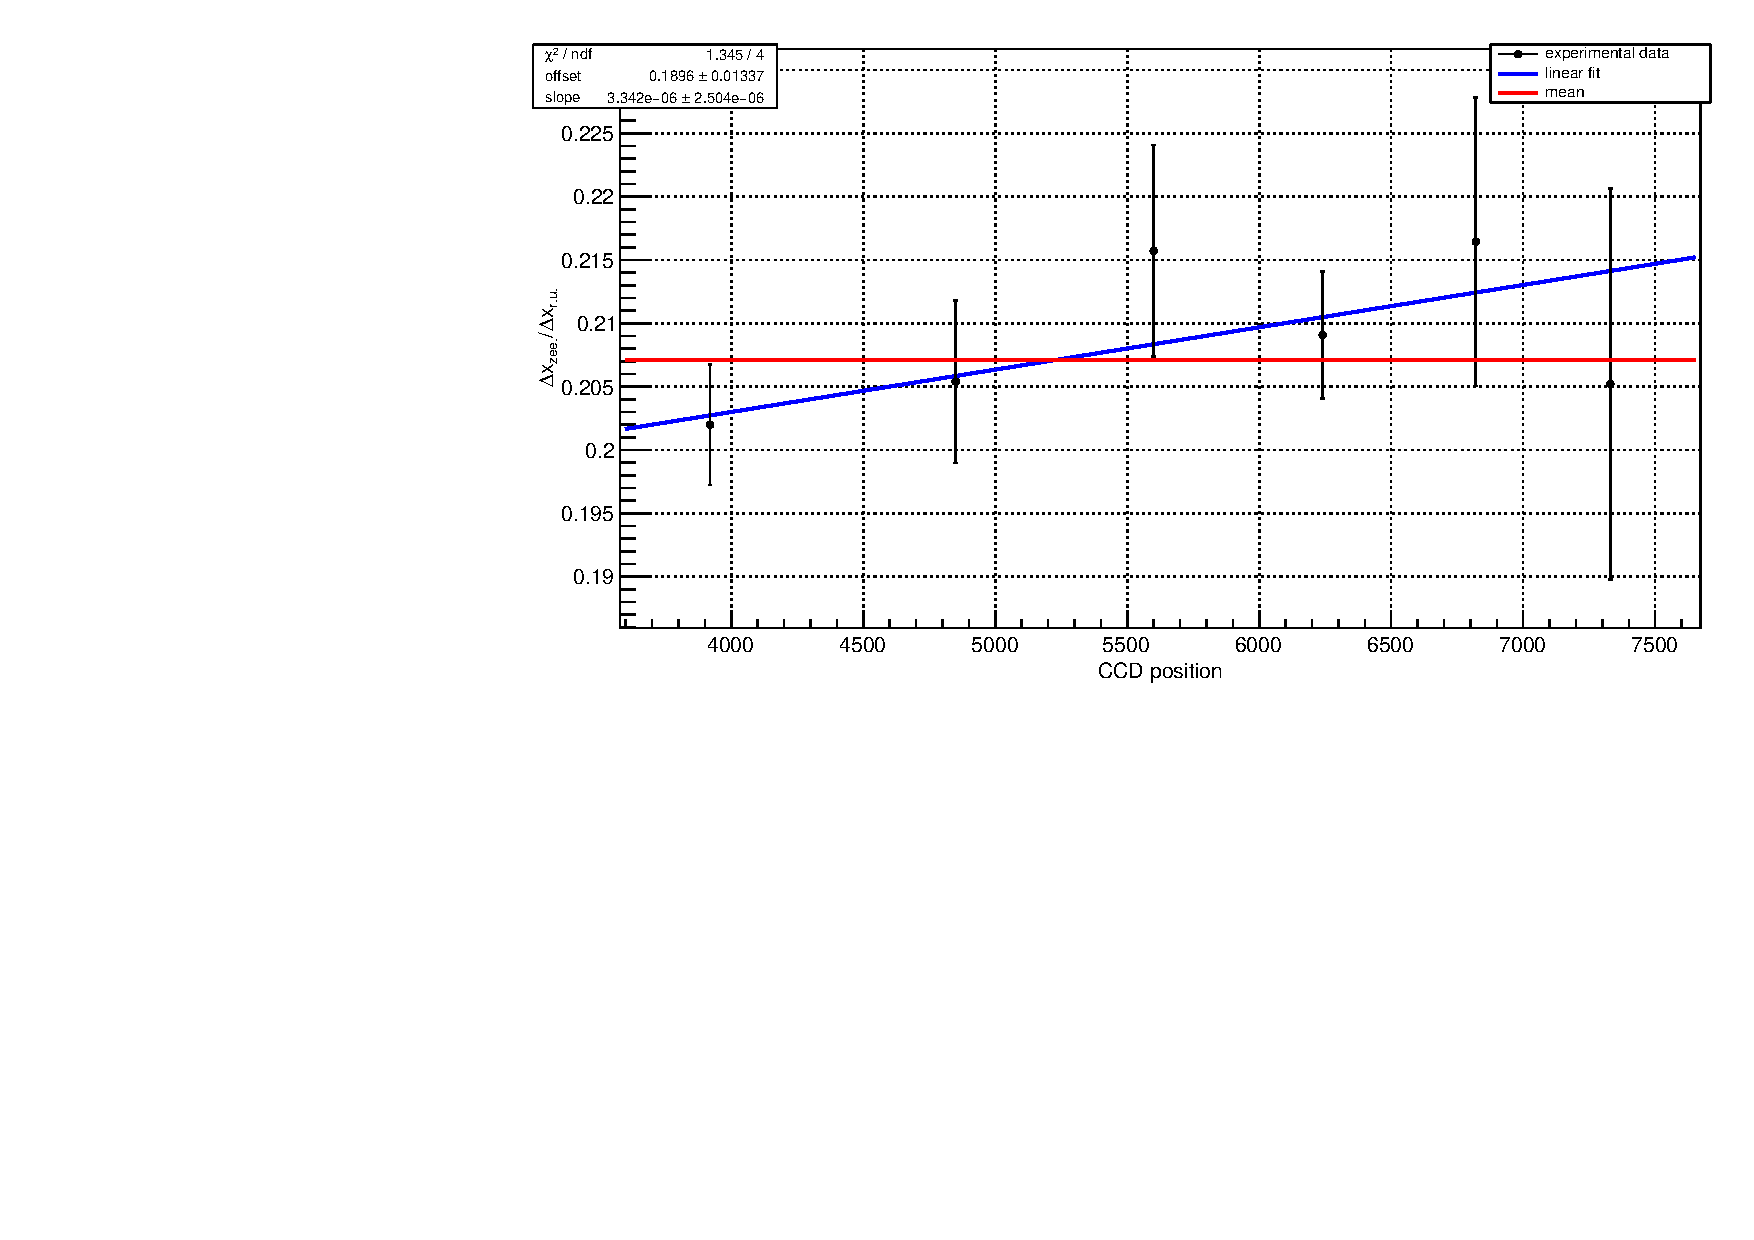
\includegraphics[scale=0.38, angle=0]{campomin/fit.pdf}
			\setlength{\belowcaptionskip}{-20pt}
			\caption{Andamento del rapporto $\Delta x_{Zee}$/$\Delta x_{ru}$}
			\label{fig:fit_rapporto_min}
		\end{figure}
	\end{center}

	\begin{center}
		\begin{figure}[H]
			\centering
			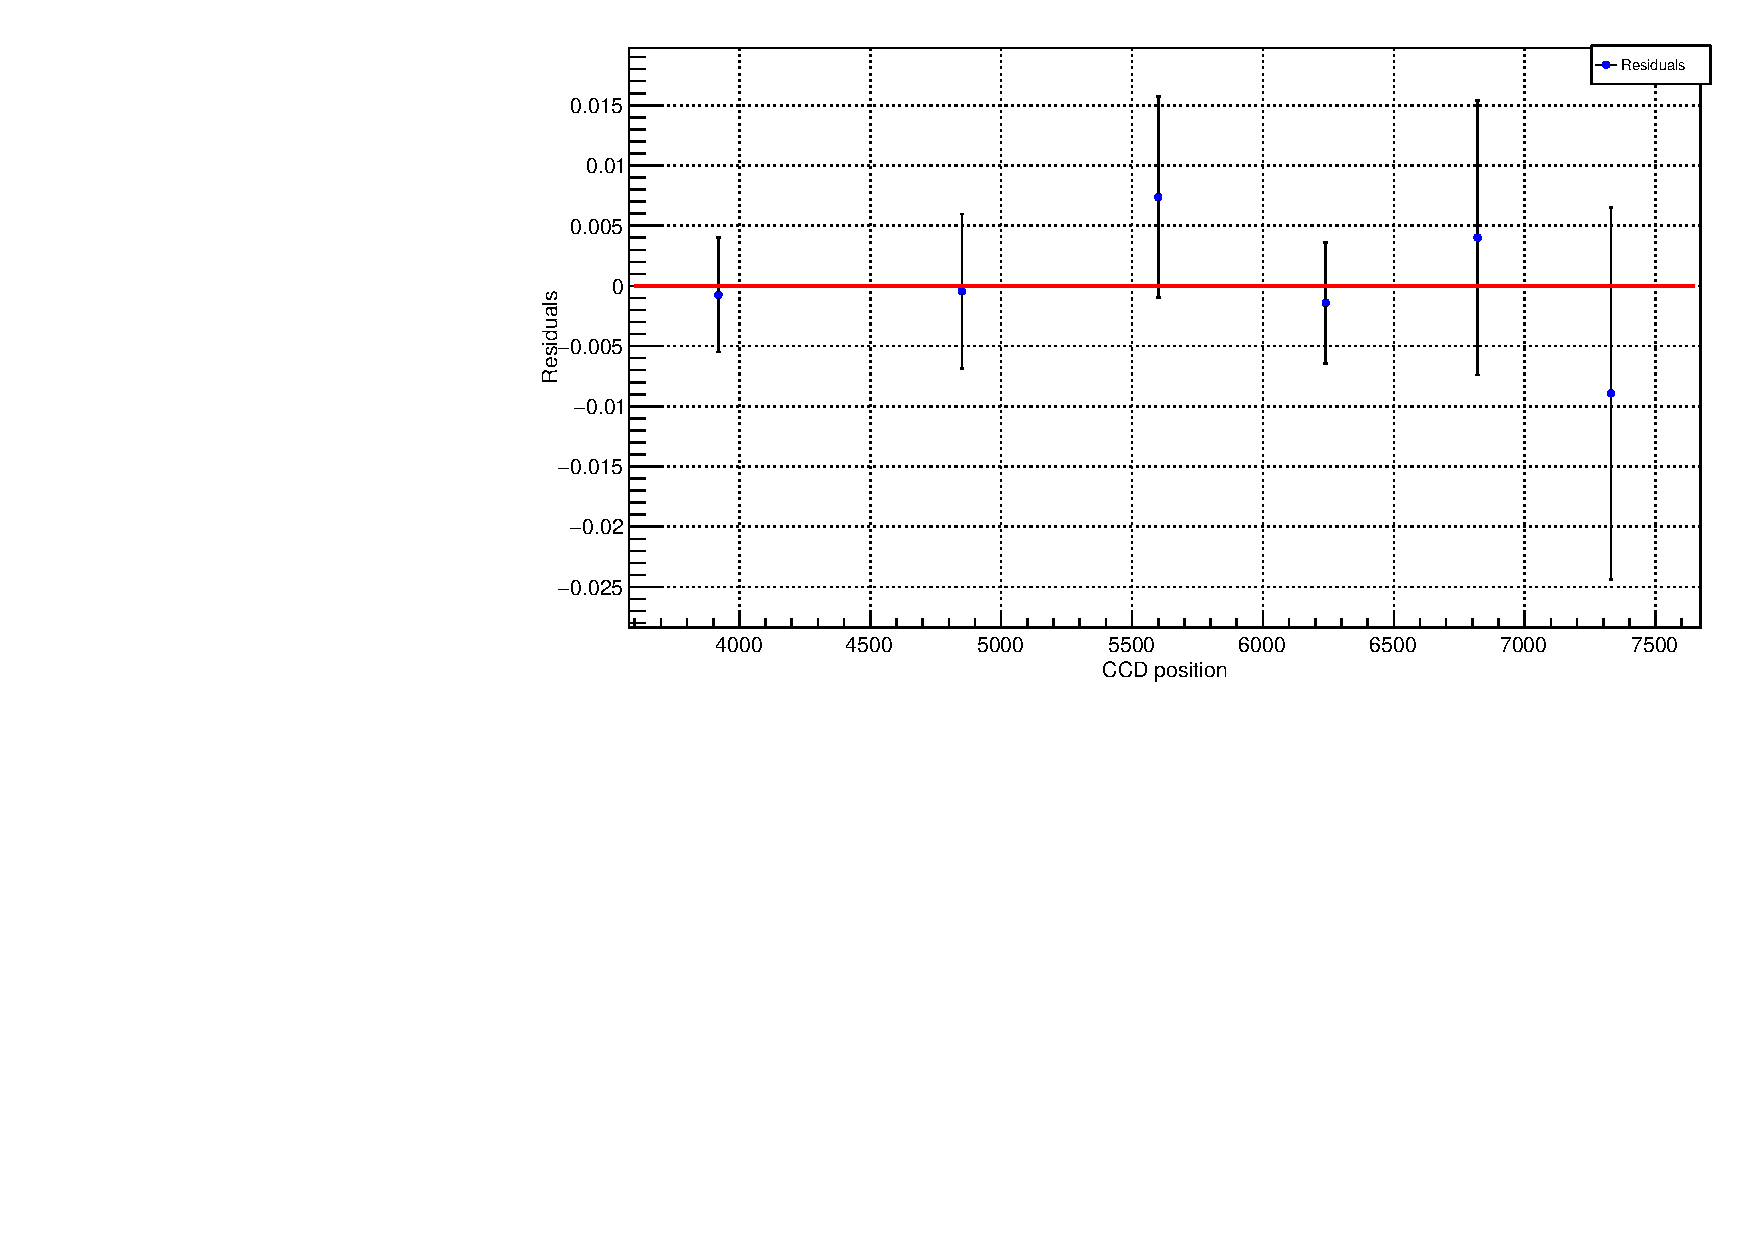
\includegraphics[scale=0.38, angle=0]{campomin/residuals.pdf}
			\setlength{\belowcaptionskip}{-20pt}
			\caption{Andamento dei residui}
			\label{fig:fit_rapporto_min_res}
		\end{figure}
	\end{center}

	La pendenza della retta con cui si è fittata la distribuzione dei rapporti è effettivamente
	compatibile con lo zero entro 2$\sigma$. Questo autorizza il calcolo della media pesata, per cui 
	la miglior stima del rapporto in questione è data da 

	\[
		\frac{\Delta x_{Zee}}{\Delta x_{ru}} = 0.207 \pm 0.003	
	\]

	Mostriamo anche un grafico equivalente con l'andamento di $\Delta\lambda_{Zee}$, ossia 
	$\Delta x_{Zee}$ opportunamente convertito con il fattore F caratteristico della relativa regione
	dello spettro.

	\begin{center}
		\begin{figure}[H]
			\centering
			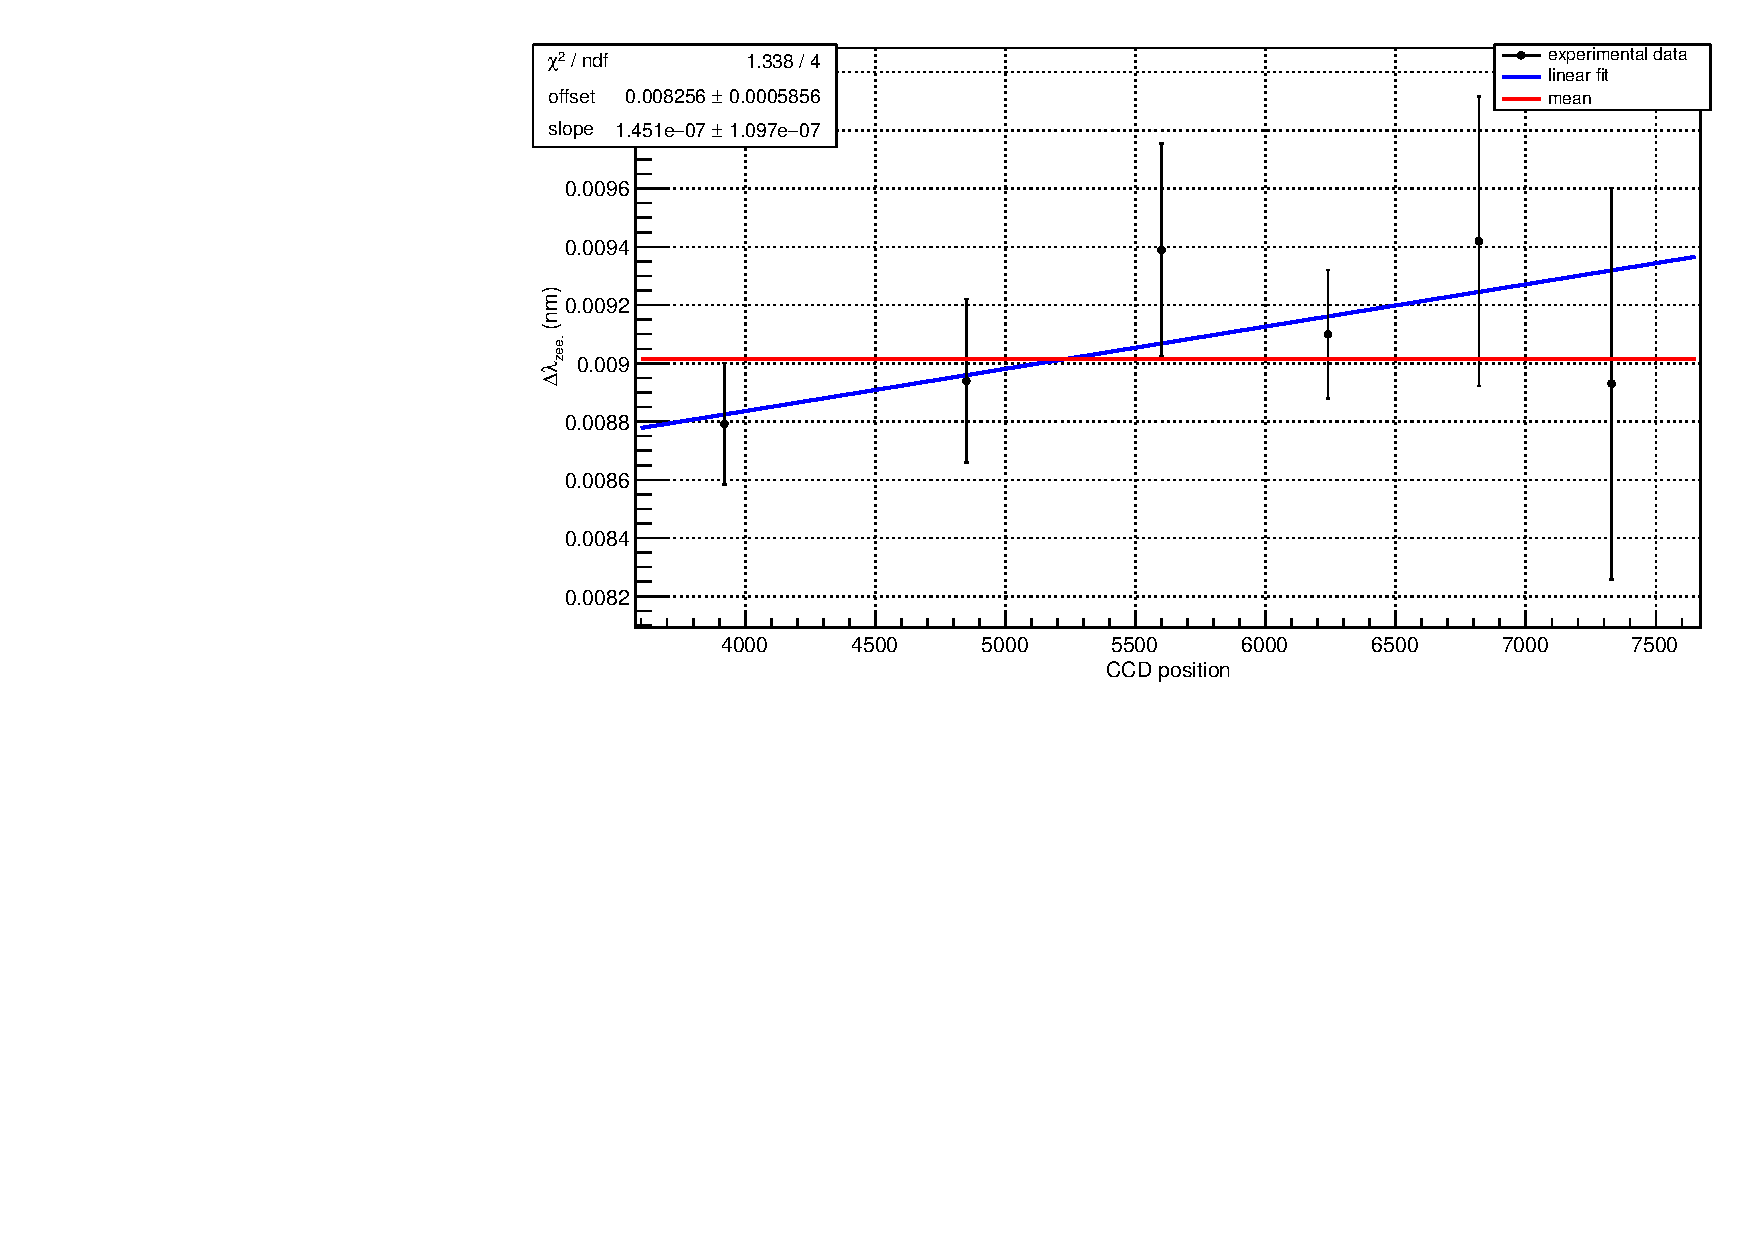
\includegraphics[scale=0.38, angle=0]{campomin/dlambdazee.pdf}
			\setlength{\belowcaptionskip}{-20pt}
			\caption{Andamento dello shifting Zeeman}
			\label{fig:fit_dlambdazee_min}
		\end{figure}
	\end{center}

	\begin{center}
		\begin{figure}[H]
			\centering
			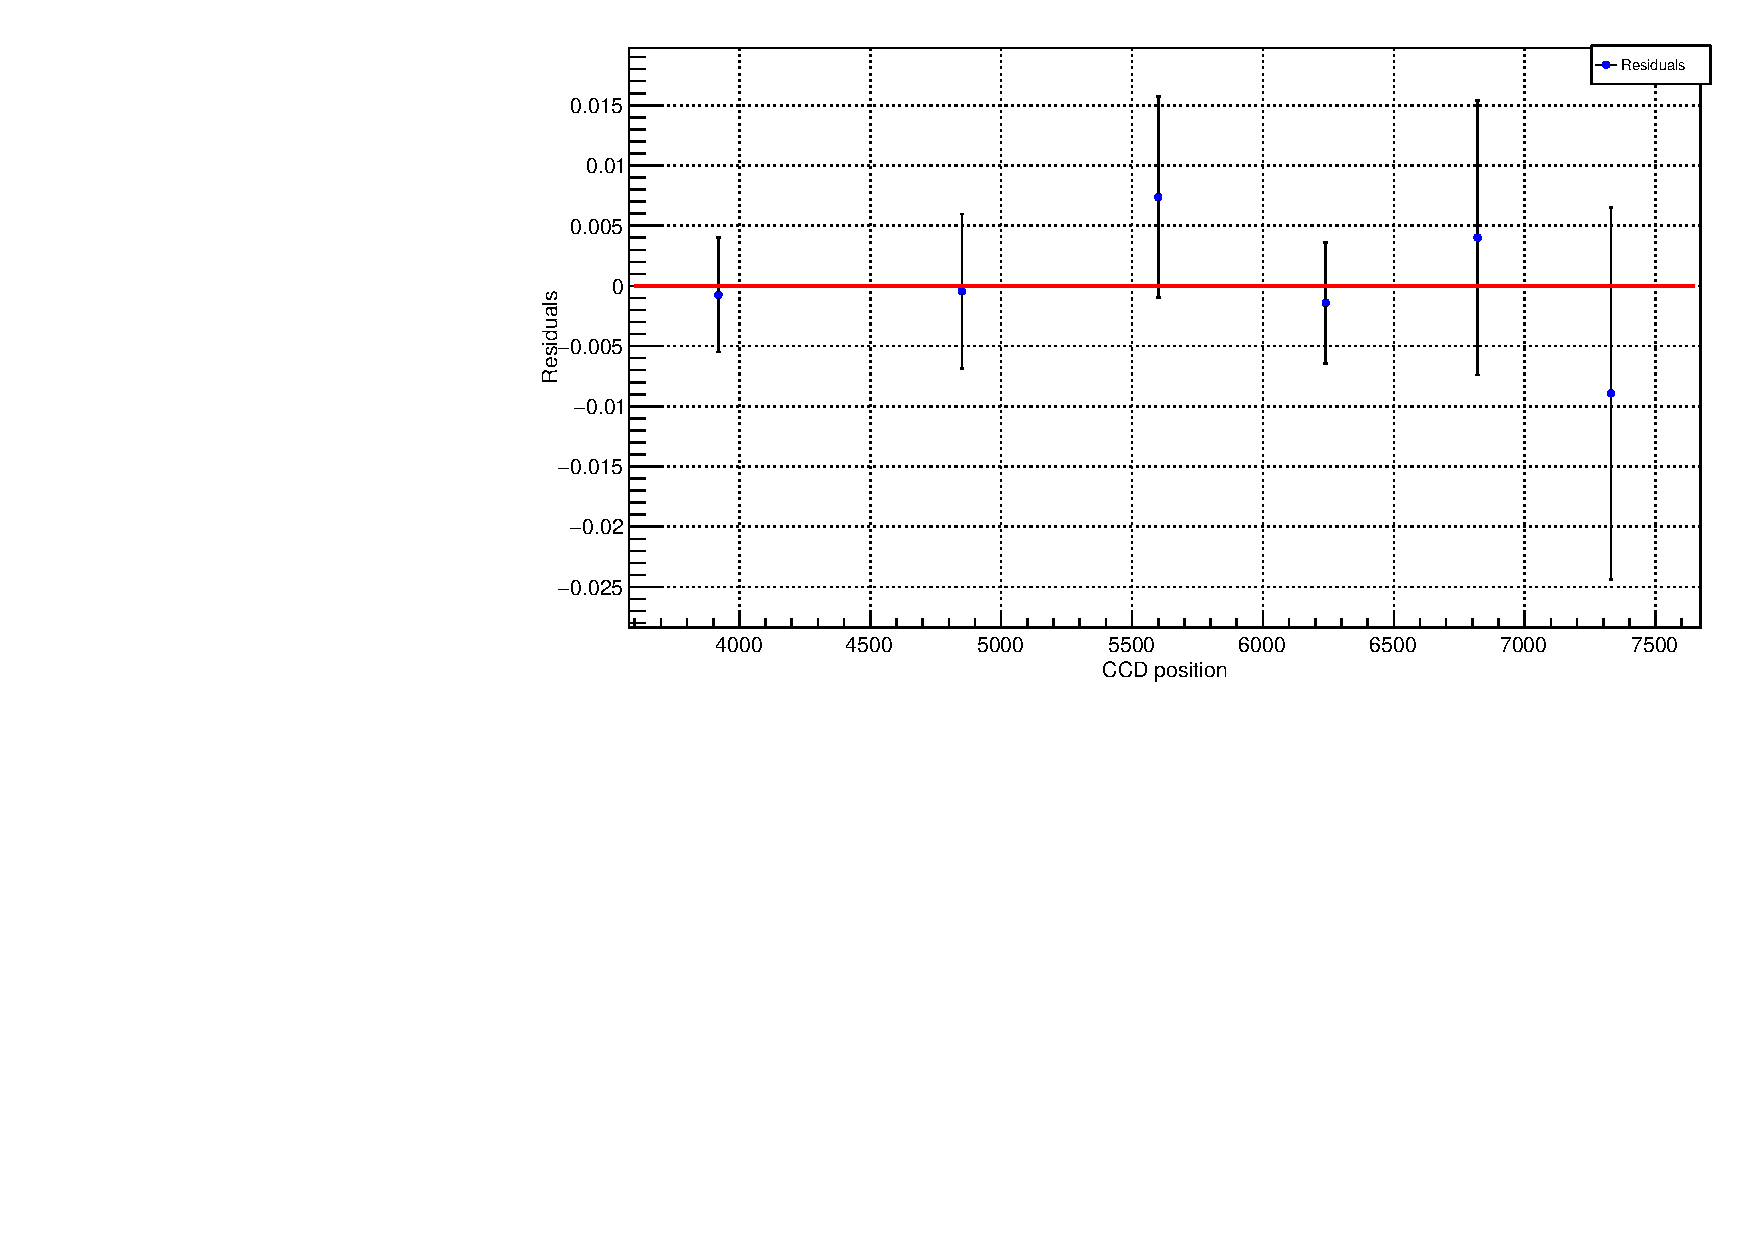
\includegraphics[scale=0.38, angle=0]{campomin/residuals.pdf}
			\setlength{\belowcaptionskip}{-20pt}
			\caption{Andamento dei residui}
			\label{fig:fit_dlambdazee_min_res}
		\end{figure}
	\end{center}

	Da cui si ricava per media pesata la miglior stima dello shifting Zeeman

	\[
		\Delta\lambda_{Zee} = (0.0090 \pm 0.0001) nm	
	\]

	che corrisponde al valore del rapporto precedentemente fornito moltiplicato per $\Delta\lambda_{ru}$.

	\begin{center}
		\begin{figure}[H]
			\centering
			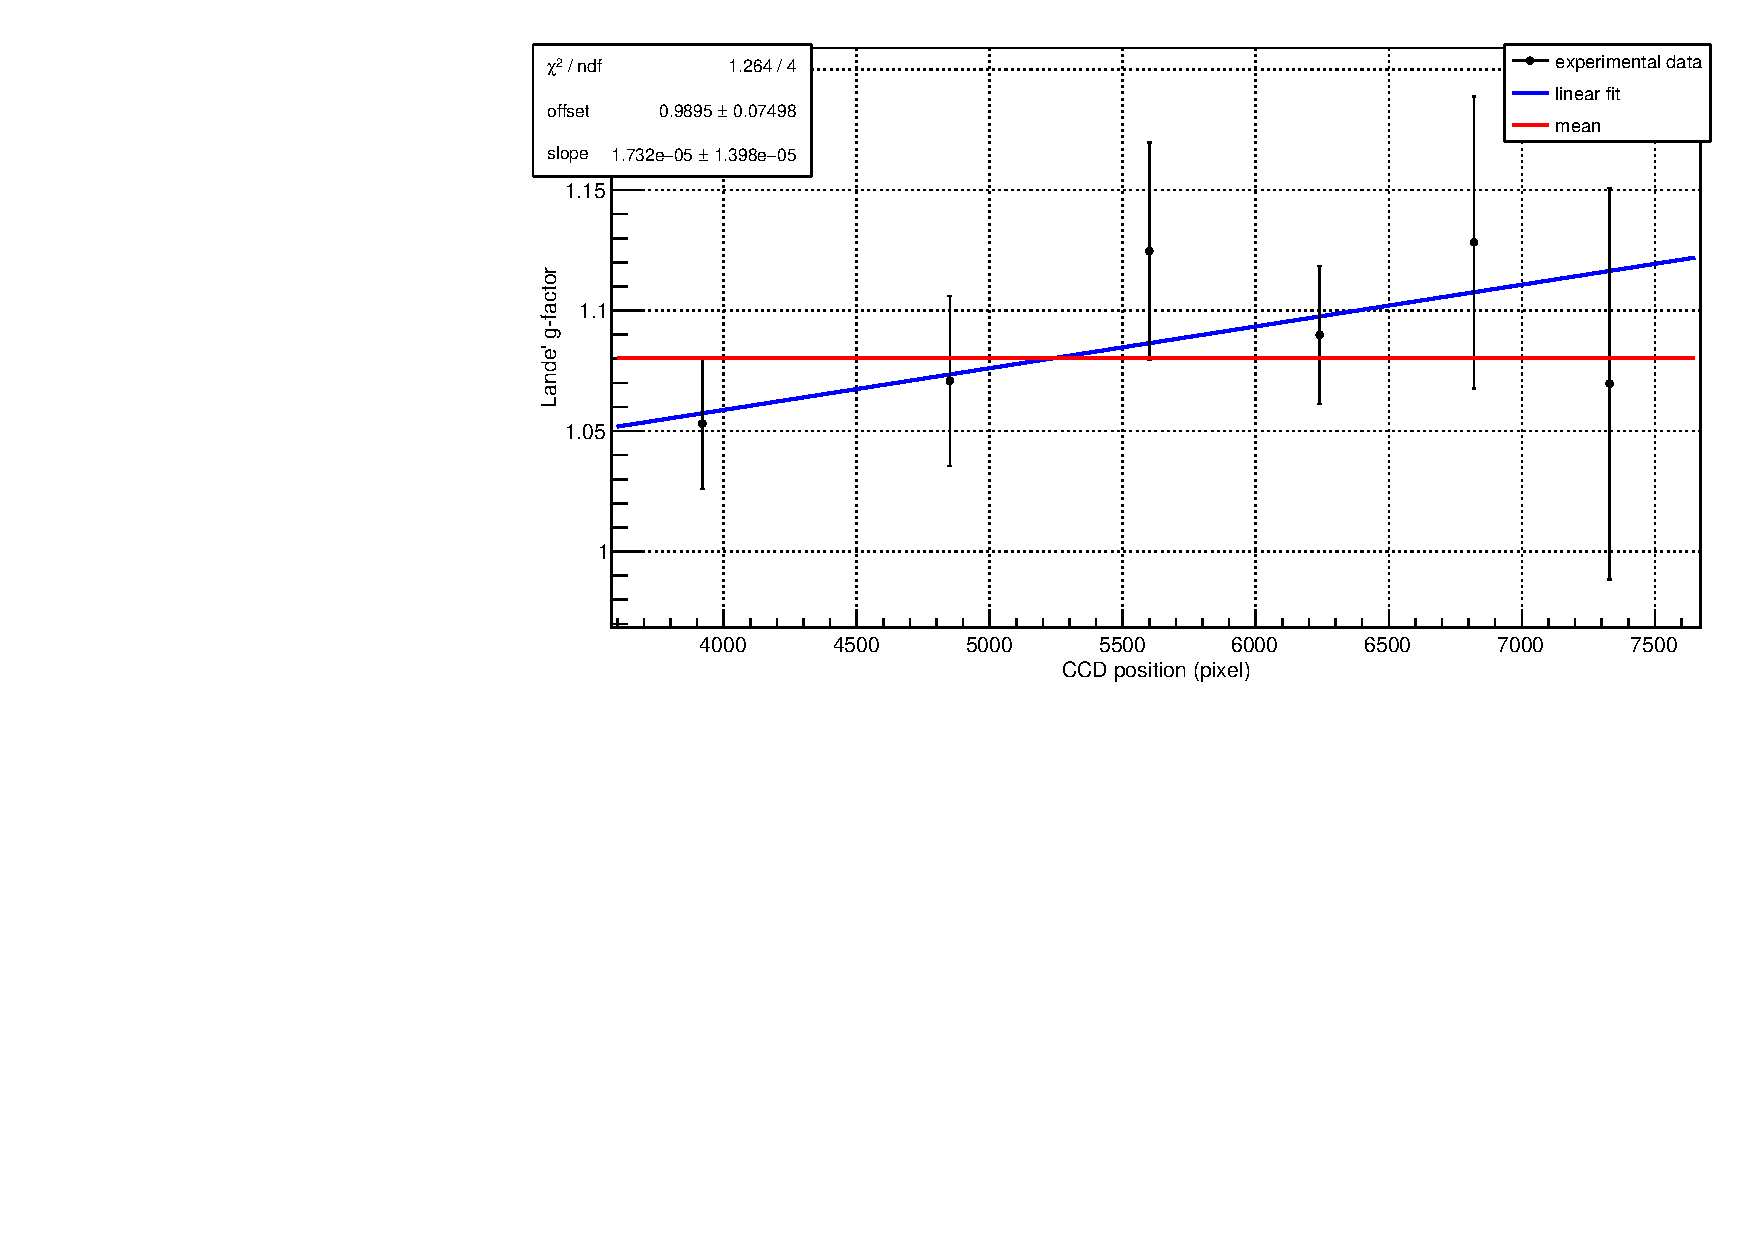
\includegraphics[scale=0.38, angle=0]{campomin/g.pdf}
			\setlength{\belowcaptionskip}{-20pt}
			\caption{Andamento del fattore giromagnetico}
			\label{fig:g_min}
		\end{figure}
	\end{center}

	\begin{center}
		\begin{figure}[H]
			\centering
			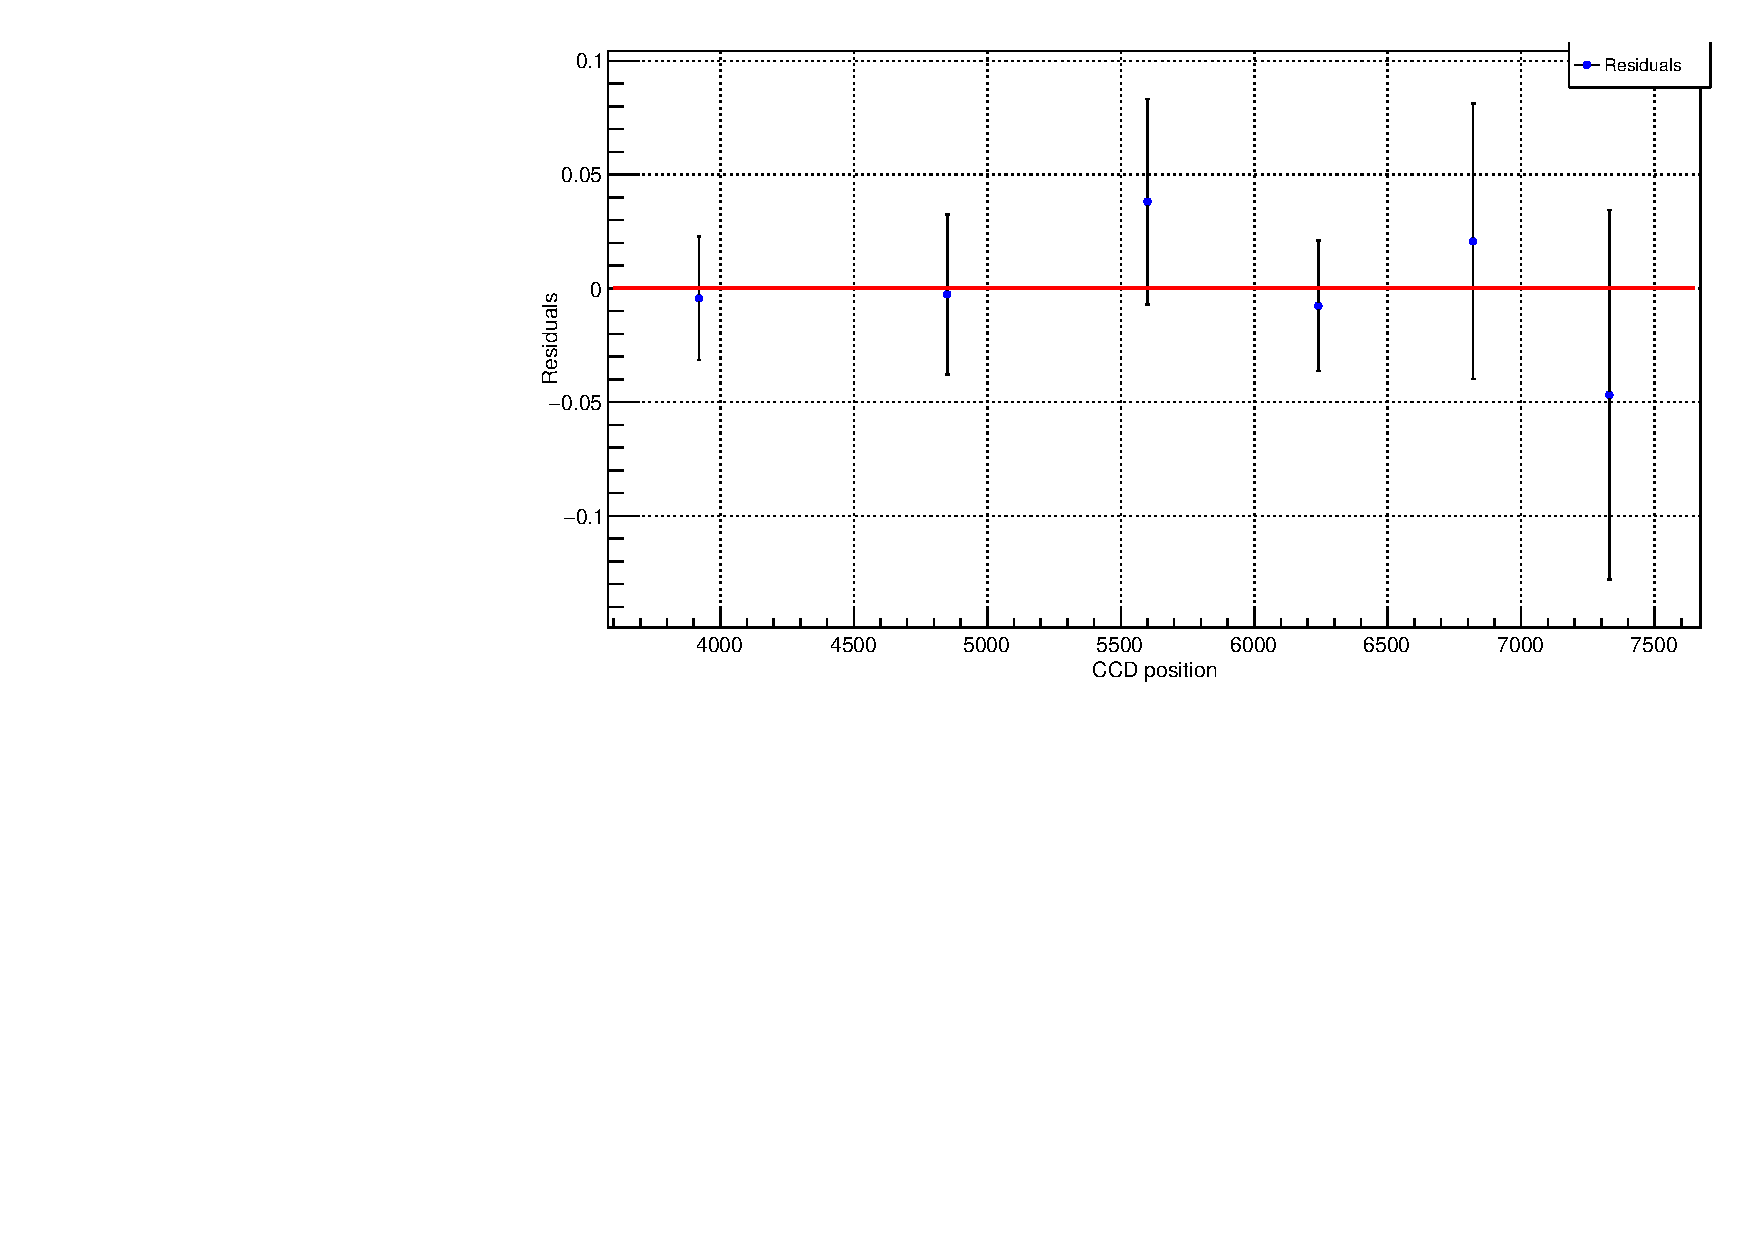
\includegraphics[scale=0.38, angle=0]{campomin/g_residuals.pdf}
			\setlength{\belowcaptionskip}{-20pt}
			\caption{Andamento dei residui}
			\label{fig:g_res_min}
		\end{figure}
	\end{center}

	Si vede subito che la pendenza del fit lineare è compatibile con lo zero entro 1$\sigma$.

	Si presenta dunque il fattore g ottenuto dal $\Delta\lambda_{zee}$ pesato.

	\[
		g = 1.08 \pm 0.02	
	\]
	
	che presenta uno scarto di circa 4$\sigma$ dal valore atteso, segno di una pessima compatibilità.

	\subsection*{Stima complessiva di g}

	Al termine dell'analisi si è quindi giunti a due stime separate di g, una proveniente dall'analisi 
	a campo massimo e una dall'analisi a campo dimezzato. Entrambe le stime di g si possono considerare
	compatibili con il valore teorico, alla luce degli scarti in $\sigma$ calcolati precedentemente. 
	La compatibilità tra i due valori sperimentali, $\lambda = 2.8$, ci permette il calcolo della media
	pesata:

	\[
		g = 1.036 \pm 0.009	\quad \sigma_{\%} = 0.88 \%
	\]



	\section*{Conclusioni}

	Il fattore giromagnetico calcolato nel caso del campo ridotto risulta impreciso e distante
	circa 4$\sigma$ dal valore atteso, come già precedentemente espresso. Pertanto la media dei due valori
	esposta poco sopra risulta difettata da tale contributo. 
	
	Alla luce di ciò si è scelto di considerare come miglior stima del valor vero il risultato figlio
	dell'analisi a campo massimo.
	Presentiamo dunque la nostra stima conclusiva

	\[
		g = 1.02 \pm 0.01	\quad \sigma_{\%} = 1.04\%
	\]
	La stima risulta soddisfare l'aspettativa teorica entro i 2$\sigma$.
	L'esclusione del fattore di campo dimezzato si può imputare a difetti strumentali, oltre che
	all'imprecisione legata a uno splitting poco definito nel caso di campo magnetico tenue, che rende 
	lacunoso il fit dei picchi.
  
 	\newpage
	\appendix
	\section{Appendici}
	\label{appendice}
	\subsection{Costruzione dell'errore sulle misure}
	\label{Calcerr}

	\subsection{Tabella delle compatibilità}
	\medskip
	\begin{table}[H]
		\centering
		\begin{tabular}{c}
			%\hline
			\begin{Large}
			$\lambda=\frac{|a-b|}{\sqrt{\sigma_a^2+\sigma_b^2}}$
			\end{Large}\\
			%\hline
		\end{tabular}
		\hspace{0.5cm}
		\begin{tabular}{cc}
			\toprule
			&       \textbf{Compatibilità   }       \\
			\midrule
			0$\leq \lambda$<1   &Ottima                 \\
			1$\leq \lambda$<2   &Buona                  \\
			2$\leq \lambda$<3   &Accettabile            \\
			3$\leq\lambda$<5   &Pessima                \\
			$ \lambda \geq $  5     &Non compatibile        \\
			\bottomrule
		\end{tabular}
		\caption{indicazioni lettura compatibilità}
		\label{tab:compatibilità}
	\end{table}
	
	
\subsection{Scelta dei ranges e principali valori }
\subsubsection{Campo spento}
\begin{center}
\begin{tabular} {ccccc}
\toprule
set	& range(pixel)& c (pixel) & F (nm/pixel)\\
\midrule
1	&	3330	-	4400	&$	364.2	\pm 0.8$& $0.0001195 \pm 5\cdot 10^{-7} $	\\
2	& 	4400	-	5250	&$	272.808 \pm 0.6$&$ 0.0001595 \pm 7\cdot 10^{-7}$ \\
3	&	5250	-	5950	&$	230.143 \pm 0.5$&$0.00018913 \pm8\cdot10^{-7}$\\
4	&	5950	-	6550	&$	202.179 \pm 0.4	$&$0.0002153 \pm 9\cdot10^{-7}$\\
5	&	6550	-	7075	&$	180.317	\pm 0.4$& $0.000241 \pm 1\cdot10^{-6} $\\
6	&	7075	-	7600	&$	165.349	\pm 0.4$& $0.000264\pm1\cdot10^{-6}$\\
\bottomrule
\end{tabular}
\end{center}

 \subsubsection{Campo acceso massimo}
\begin{center}
\begin{tabular} {ccccc}
	\toprule
set	& range (pixel)& $\Delta\lambda_{Zee} $ (nm) & g \\
\midrule
1	&	3330	-	4400	&  $0.0161 \pm  1\cdot 10^{-4}$	&$1.02 \pm 0.01$\\  
2	& 	4400	-	5250	&  $0.01604 \pm 9\cdot 10^{-5}$&$1.01 \pm0.01$\\ 
3	&	5250	-	5950	&	$0.01602 \pm 9\cdot10^{-5}$&$1.01 \pm 0.01$\\
4	&	5950	-	6550	&	$0.0163 \pm 1\cdot 10^{-4}$&$1.03 \pm 0.01$\\
5	&	6550	-	7075	&	$0.0163 \pm1\cdot 10^{-4}$&	$1.03  \pm 0.01$	\\
6	&	7075	-	7600	&	$0.0161\pm1\cdot 10^{-4}$&	$1.02 \pm 0.01$	\\
\bottomrule
\end{tabular}
\end{center}

 \subsubsection{Campo acceso dimezzato}
\begin{center}
	\begin{tabular} {ccccc}
		\toprule
		set	& range (pixel)& $\Delta\lambda_{Zee} $ (nm) & g \\
		\midrule
		1	&	3330	-	4400	&  $    0.009 \pm  0.0002$	&$1.05 \pm 0.03$\\  
		2	& 	4400	-	5250	&  $0.0089 \pm 0.0003$&$1.07 \pm0.04$\\ 
		3	&	5250	-	5950	&	$0.0094\pm 0.0004$&$1.12 \pm 0.05$\\
		4	&	5950	-	6550	&	$0.0091\pm 0.0002$&$1.09 \pm 0.03$\\
		5	&	6550	-	7075	&	$0.0094 \pm0.0005$&	$1.13 \pm 0.06$	\\
		6	&	7075	-	7600	&	$0.0089\pm 0.0007$&	$1.07 \pm 0.08$	\\
		\bottomrule
	\end{tabular}
\end{center}
   
\end{document}
